% TODO JAMES where to write more? which sections are weakest? (more code?)
% TODO JAMES O runtime online is different to empirical findings
% TODO CHECK is "classification accuracy" correct?

% TODO END add "recall that"
% TODO NOW rename slice optimisation
% TODO END always mention name when you cite
% TODO for acquisition function: describe a hat for samples
% TODO maybe switch from "score" to "error"
% TODO CITE http://mlg.eng.cam.ac.uk/hoffmanm/papers/hoffman:2014.pdf
% TODO END remove todos from code
% TODO END citations: switch to different format, make sure author is mentioned, If you use purely-numeric bibliographic references, do not forget to still mention authors’ surnames
% TODO convert sparse arff files to non sparse
% TODO rnd forest is bad at data that's heavily pos or neg, run tests
% TODO END random forest(s) spelling
% TODO END dataset /data set spelling
% TODO END abkürzungsverzeichnis
% TODO END performance/time/accuracy, be clear
% TODO END run time spelling
% TODO END explain score and 1-score, more natural to think in terms of improvement
% TODO END trade-off spelling
% TODO http://www.springer.com/gp/book/9783540653677
% TODO END "n't" -> "not"
% TODO END refer to sections, not chapters (as numbers)
% TODO possible goal: fixed error, trade off data and time
% TODO END don't talk about "subsection", subsub...
% TODO END emph new definitions
% TODO END use "equation" instead of equation* (also align)
% TODO END figure/Figure capitalisation
% TODO END capitalisation of chapters/sections
% TODO END no arxiv references
% TODO END percentage of data values, consistent term
% TODO END present/past
% TODO UML diagram for schedulers
% TODO describe kernel problems
% TODO END check for emotional language
% TODO datasets: http://rodrigob.github.io/are_we_there_yet/build/classification_datasets_results.html
% TODO explain datasets w/ images if they are interesting
% TODO explain how exponential growth is at most 2x as bad as 100%
% TODO the field of "sequential analysis"
% TODO mention bounds as alternative to EI
% TODO cite http://www.cs.ubc.ca/~poole/papers/randaccref.pdf
% TODO END no footnotes or cites after formulas
% TODO END random forest(s) consistent plural/capitalisatino (also logreg)

\documentclass[a4paper,12pt,twoside,openright]{report}

% Diagrams
\usepackage{graphicx}

\def\authorname{Jan S\"ondermann\xspace}
\def\authorcollege{Selwyn College\xspace}
\def\authoremail{jjes2@cam.ac.uk}
\def\dissertationtitle{Bayesian optimisation of approximateness in the trade-off between statistical and computational efficiency}
% TODO END word count
\def\wordcount{@}

\usepackage{euscript}
\usepackage[export]{adjustbox}
\usepackage{subcaption}
\usepackage{chngpage}
\usepackage{calc}
\usepackage{epsfig,graphicx,parskip,setspace,tabularx,xspace} 
\usepackage{enumitem}
\usepackage{mathtools}
\usepackage{amsmath,amssymb}
\usepackage{algorithmicx}
\usepackage{algorithm}
\usepackage{algpseudocode}
\newcommand{\Break}{\State \textbf{break} }
\usepackage{listings}
\lstset{breaklines=true, frame=single, numbers=left, basicstyle=\small\ttfamily}

\DeclareMathOperator*{\argmax}{arg\,max}


%% START OF DOCUMENT
\begin{document}


%% FRONTMATTER (TITLE PAGE, DECLARATION, ABSTRACT, ETC) 
\pagestyle{empty}
\singlespacing
% title page information
\begin{titlepage} 

\begin{center}
\noindent
\huge
\dissertationtitle \\
\vspace*{\stretch{1}}
\end{center}

\begin{center}
\noindent
\huge
\authorname \\
\Large
\authorcollege      \\[24pt]

\includegraphics{CUni3.eps}
\end{center}

\vspace{24pt} 

\begin{center}
\noindent
\large
{\it A dissertation submitted to the University of Cambridge \\ 
in partial fulfilment of the requirements for the degree of \\ 
Master of Philosophy in Advanced Computer Science} 
\vspace*{\stretch{1}}
\end{center}

\begin{center}
\noindent
University of Cambridge \\
Computer Laboratory     \\
William Gates Building  \\
15 JJ Thomson Avenue    \\
Cambridge CB3 0FD       \\
{\sc United Kingdom}    \\
\end{center}

\begin{center}
\noindent
Email: \authoremail \\
\end{center}

\begin{center}
\noindent
\today
\end{center}

\end{titlepage} 

\newpage
\vspace*{\fill}

\onehalfspacing
\newpage
{\Huge \bf Declaration}

\vspace{24pt} 

I \authorname of \authorcollege, being a candidate for the M.Phil in
Advanced Computer Science, hereby declare that this report and the
work described in it are my own work, unaided except as may be
specified below, and that the report does not contain material that
has already been used to any substantial extent for a comparable
purpose.

\vspace{24pt}
Total word count: \wordcount

\vspace{60pt}
\textbf{Signed}: 

\vspace{12pt}
\textbf{Date}:


\vfill

This dissertation is copyright \copyright 2010 \authorname. 
\\
All trademarks used in this dissertation are hereby acknowledged.



\newpage
\vspace*{\fill}

\singlespacing
\newpage
{\Huge \bf Abstract}
\vspace{24pt} 


% TODO write abstract
%Our project falls into the field of meta-machine learning that tries to use machine learning methods to improve the result of using these methods.


\newpage
\vspace*{\fill}


Our project falls into the field of meta-machine learning that tries to use machine learning methods to improve the result of using these methods.

\pagenumbering{roman}
\setcounter{page}{0}
\pagestyle{plain}
\tableofcontents
\listoffigures
\listoftables

\onehalfspacing

%% START OF MAIN TEXT 

\chapter{Introduction}
% TODO add citations

\pagenumbering{arabic}
\setcounter{page}{1}
% TODO explain that we need not only be fast when optimising but are also constrained by the time budget (need to finish in time)

Before the advent of computers, statistical methods had to be simple enough to be calculable by hand which greatly limited the degree of complexity that these methods could reach. As computing power available to statisticians increased, many new methods were devised to make use of these new resources. In some cases, these new methods even exceed the computational possibilities and are computationally intractable. 

Although machine learning is a very diverse subject that combines influences from many different fields such as engineering, computer science, computational biology and physics, many of the recent advances have come from statistics or made use of statistical methods. As is true for mathematics more generally, considerations of run time and complexity are usually not in the focus of attention of statistical research. 

% TODO instead of burden -> jordan: workload
The cultural differences between computer science and statistics is revealed in the attitudes towards data that these fields exhibit: while in computer science, more data is viewed as a "burden", something negative to be brought under control, in statistics, the perception is that more data is desirable as it allows higher confidence in inferential results.

Public perception of machine learning has concentrated on the rapid growth of data to be analysed, a phenomenon often called "Big Data". This development has made issues of run time become increasingly acute. 

The current states of the field of machine learning requires skilled humans to make high level decisions on trade-offs between computational and statistical efficiency such as when to use approximate inference methods or when to use a simple method with lots of data rather than a complex method with a small amount of data. The knowledge necessary to make adequate decisions in these cases is often acquired through experience and an intuitive familiarity with the learning algorithms that can be hard to formalise and teach.

% cite auto. stat./auto weka
As part of the current trend to automise all aspects of machine learning, automating the process of finding a balance in these trade-offs would make an important contribution to the field. Finding this balance can be seen as an optimisation problem that optimises the function from a number of "approximation parameters" to the time and prediction performance of the learning algorithms. 

Classical optimisation methods may be ineffective as solutions to this problem as evaluating the function to be optimised can be very expensive to compute. Further complicating this problem is the fact that the time required to evaluate the function can vary drastically depending on where it is evaluated: consider the case where the approximation parameter is the number of layers in a deep neural network. Increasing the number of layers will cause the inference to take more time. The optimisation routine has to take this into account when exploring the function. A natural solution to this problem is Bayesian optimisation as Bayesian optimisation methods make very efficient use of data when optimising a function.

% TODO MAYBE cite http://rbr.cs.umass.edu/papers/ZCCijcai99.pdf
% TODO EDIT make the goals clear. maybe just two, anytime and contract
Adding run time considerations to statistical learning methods can lead to a number of different goals. One possible goal are anytime algorithms that can be interrupted while running, returning a solution optimal for the amount of time they were allowed to run for. Another goal is to develop contract algorithms that receive a data set and a time budget as input and infer an optimal model within the time budget.

% TODO is this true?
%In this project, we develop a system that @. As neither of these two problems has an analytic solutions, we wrote a number of heuristics that use Bayesian optimisation methods to decide @.

% TODO EDIT second major contribution ne?
Our first major contribution in this project is a model of the function from approximation parameters to learning algorithm performance. This is the foundation for the second major part of our system which consists of a number of heuristics that use the model as a basis for Bayesian optimisation. Because these heuristics try to find an optimal evaluation sequence for the function to be optimised, we call them "schedulers".

\begin{figure}
\centering
  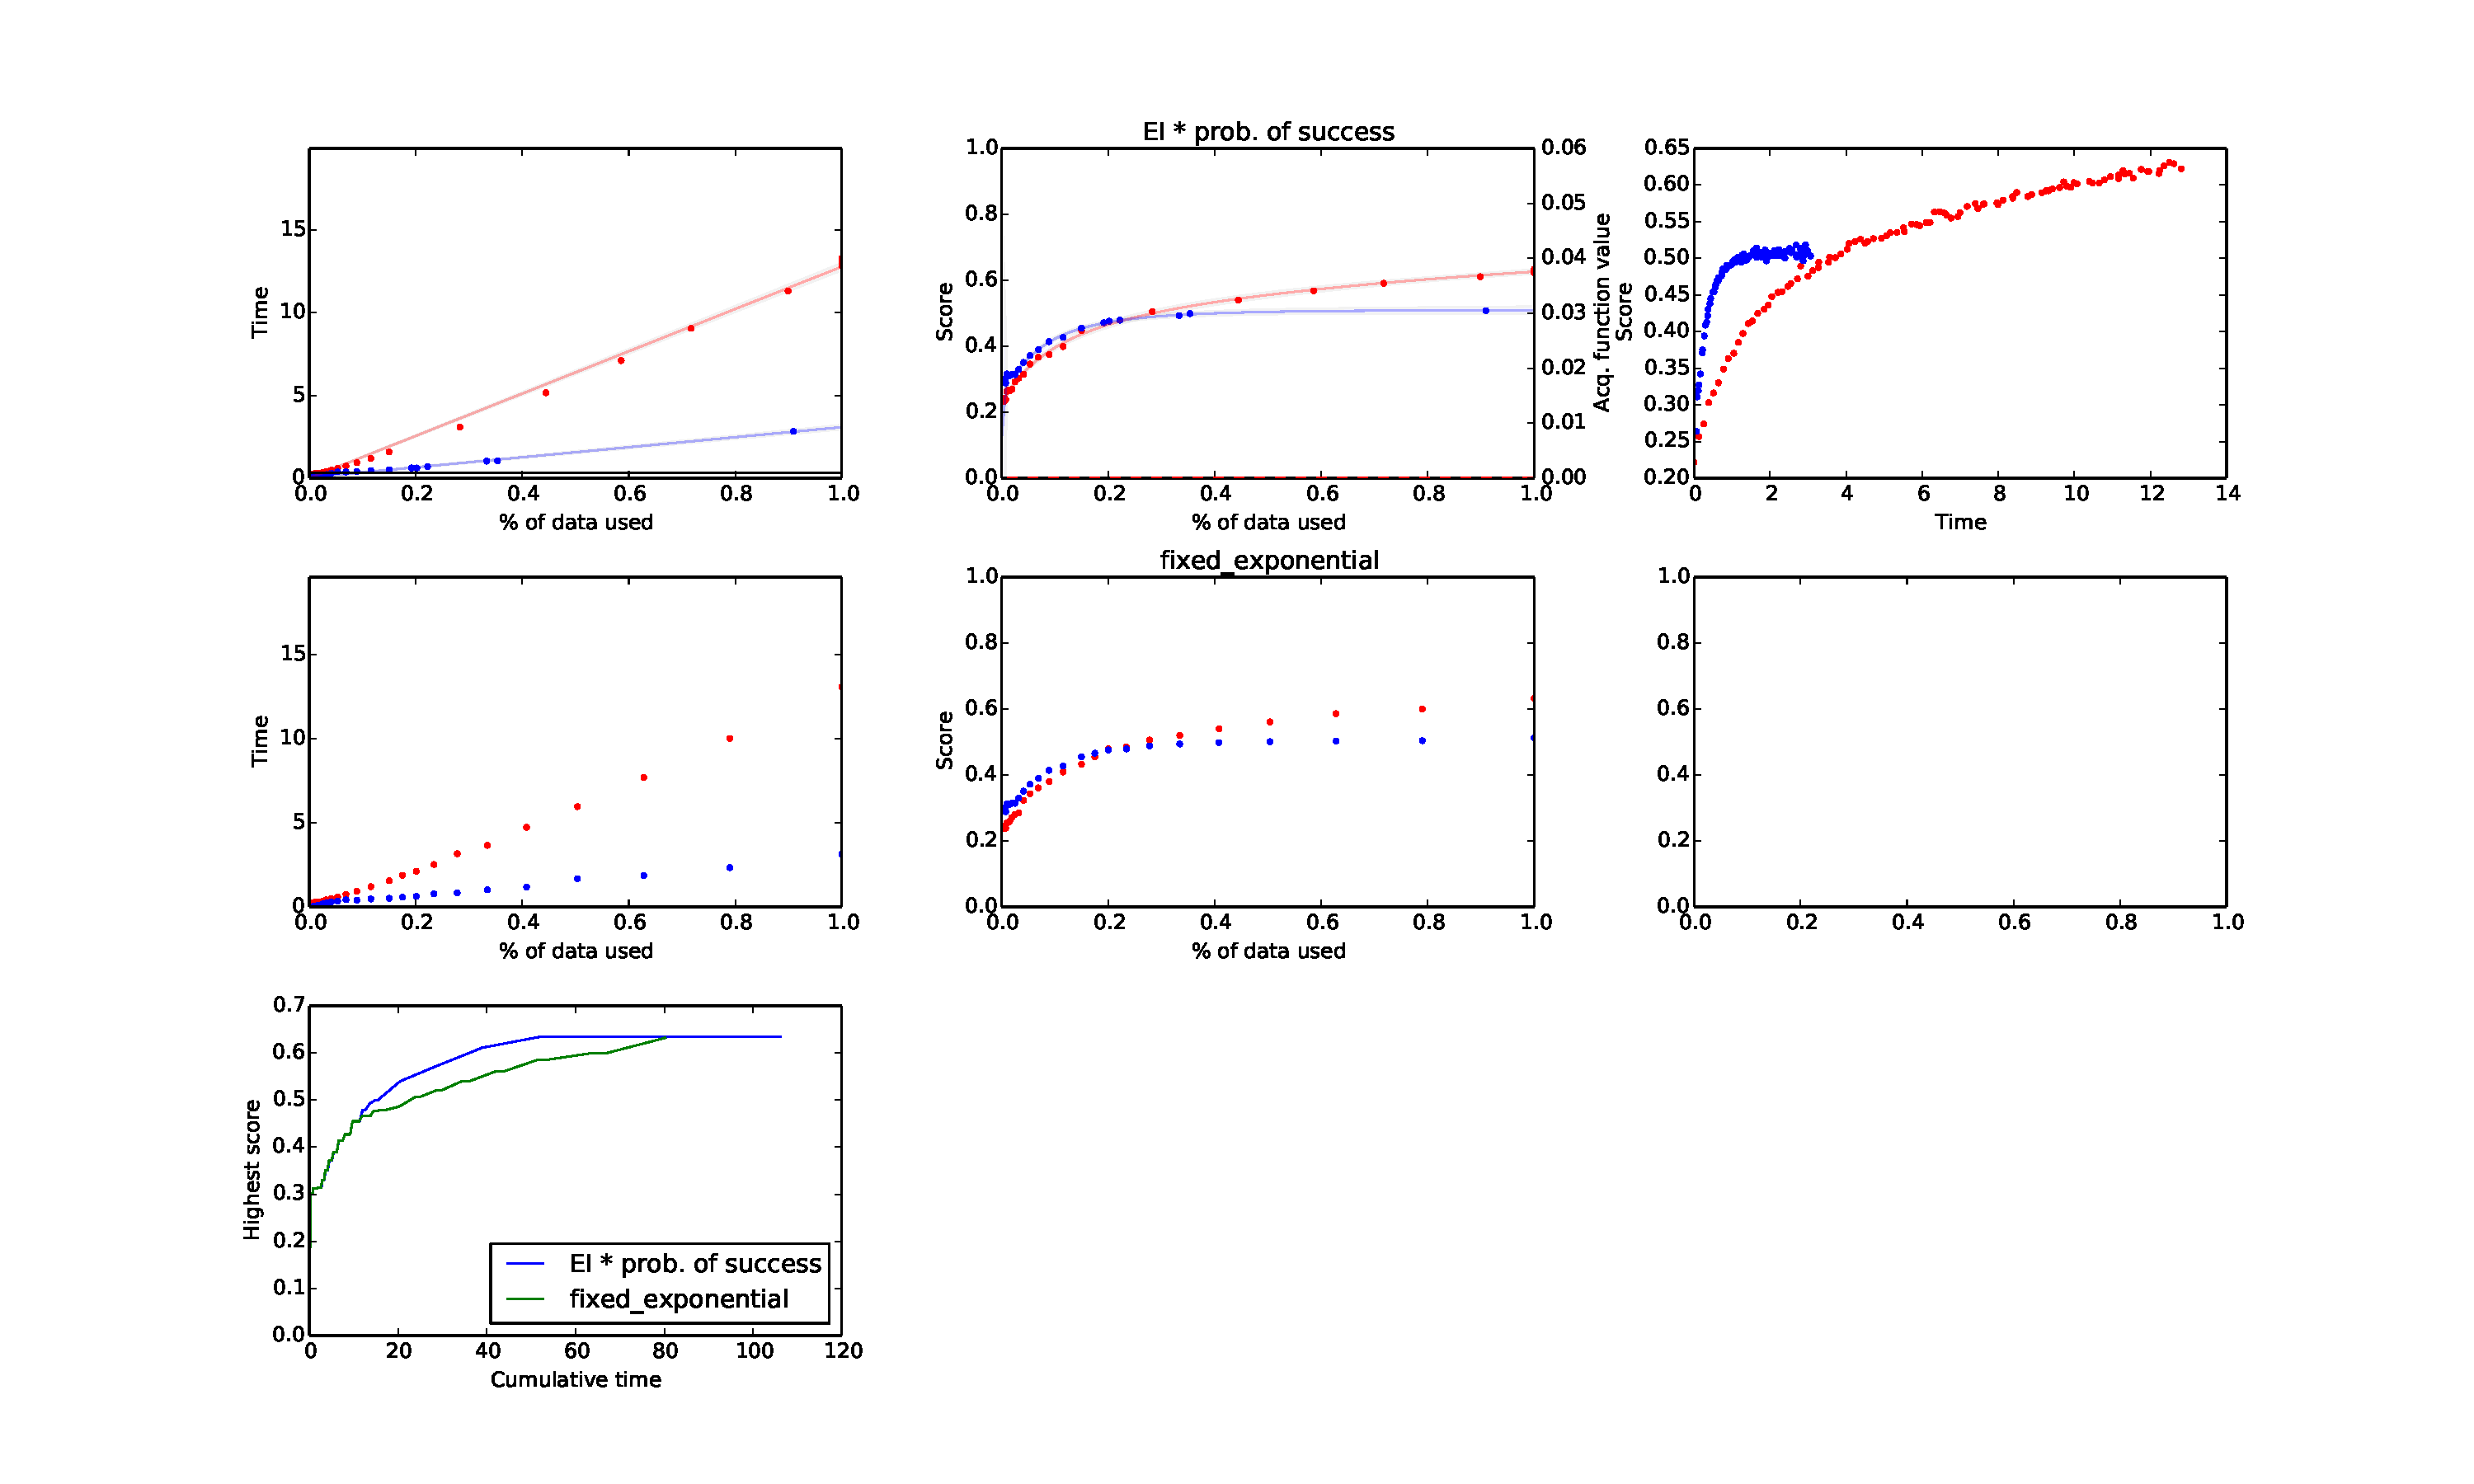
\includegraphics[trim=130 40 910 560,clip,width=\textwidth]{figures/anytime1.pdf}
  \caption{Comparing two schedulers}
  \label{anytime1}
\end{figure}

% TODO add . to prob
Figure \ref{anytime1} shows a plot that compares the performance of two such schedulers. The x-axis shows the time in seconds that the scheduler has been allowed to spend searching for the best model while the y-axis shows the classification accuracy of the best model the scheduler has found. The "\texttt{fixed\_exponential}" scheduler is a naive implementation that simply tries a fixed sequence of values for the approximation parameter. The "\texttt{EI * prob of success}" scheduler is a heuristic we developed to approximate an anytime algorithm. Both schedulers spend about 10 seconds in a burn-in phase. After this burn in ends, the blue scheduler immediately starts dominating the green scheduler and plateaus out at the maximum value about 50 seconds after learning starts. To reach the same classification accuracy, the naive scheduler needs about 80 seconds.

Although eventually both schedulers reach the same final accuracy, if we terminate both schedulers after 30 seconds, the best model found by the "\texttt{EI * prob of success}" is substantially better than that found by the naive scheduler at this point. It is therefore a heuristic for an anytime algorithm.

The rest of this dissertation is structured as follows:
\begin{itemize}
	\item The \textbf{Background} chapter introduces the theoretical ideas that this project is built on. It also lists the third-party technologies that were used during development
	\item The \textbf{Related Work} summarises the current state of research regarding the problems we are trying to solve
	\item The \textbf{Design and Implementation} chapter explains the features of our system, starting with a high level overview and continuing to a detailed description
	\item The \textbf{Evaluation} section critically examines what we have built by testing the system and evaluating results. It also lists challenges we faced and limitations of our current implementation
	\item The \textbf{Conclusion and future work} recapitulates our results by returning to the broader context lined out in this introduction and lists possible ways of extending the existing system
\end{itemize}












\chapter{Background}
% TODO A more extensive coverage of what's required to understand your work. In general you should assume the reader has a good undergraduate degree in computer science, but is not necessarily an expert in the particular area you've been working on. Hence this chapter may need to summarise some ``text book'' material. 
\textit{This chapter describes the background assumed in the remainder of the document. We give a brief explanation of general machine learning principles together with a summary of the algorithms used. We then describe the datasets we used during the course of the project.}





\section{General machine Learning concepts}
\begin{figure}
\centering
  \includegraphics[width=.8\textwidth]{figures/ml.pdf}
  \caption{The general process of learning from data}
  \label{mlstructure}
\end{figure}

\section{Key concepts}
Our project falls into the field of meta machine learning. We use machine learning algorithms to learn and predict the performance of other machine learning algorithms. This necessitates a very brief overview of machine learning principles. Figure \ref{mlstructure} shows the general structure of learning from data: a learning algorithm takes some training data and outputs a function $\hat{f}$, usually called a model of the data, that models the true function $f$ underlying the data. This function is then used to make predictions on unseen data.

Of particular relevance to our project is the second input to the learning algorithm: its hyperparameters. These hyperparameters control the behaviour of the learning algorithm and influence the quality of the model which makes selecting appropriate hyperparameters crucial.


\subsection{Approximation parameters}
By "approximation parameters", we denote parameters to machine learning algorithms that influence the trade-off between statistical and computational efficiency, letting us vary the degree of approximateness at which the algorithm runs. Changing an approximation parameters should either decrease the run time at the cost of classification accuracy or improve accuracy while making training slower. 

The approximation parameter that we put most of our focus on in this project is the proportion of the available data. Other approximation parameters are hyperparameters to the machine learning algorithms such as the number of decision trees in a random forest. These parameters are considered in the modelling chapter to analyse how multiple interaction parameters interact.

Note that not all hyperparameters are approximation parameters. Some hyperparameters influence performance without changing the run time such as the length-scales of Gaussian process kernels, explained in depth in the Gaussian process section of this chapter.\footnote{Many machine learning packages include parameters such as the number of threads used for learning in their API. These are parameters that influence run time but not performance. They are, however, particular to the implementation and not part of the algorithm.}

% TODO why did you select the appr params you selected, later you only use data. data is enough to be interesting but we want to show that approach can in principle be extended

% TODO make a table that lists approx prarms and approx params that are 

\subsection{Scheduling}
As mentioned in the introduction, the problem we try to solve in this project is an optimisation problem with the additional component of running time constraints. A solution to this problem consists in devising strategies to decide on a sequence of evaluations of the function to be optimised such that we find an optimum within these constraints. 

We use the term "scheduler" to denote heuristics that decide on such a sequence. Schedulers allocate the time available for optimisation to the possible algorithm and hyperparameter combinations.

\section{Machine learning algorithms}
\subsection{Logistic regression and random forest}
% TODO mention that you focus on rnd-forest/log-reg and data only
This subsection introduces the two machine learning algorithms that we focus on in the evaluation of our system, random forest and logistic regression. Both of these algorithms are among the most common machine learning algorithm and are frequently used in real world applications. % cite

% TODO important to introduce algos to understand appr params
% TODO talk about what each algorithm is good/weak at

\subsubsection{Logistic regression}
% TODO in linear regression, are more complex base functions used
Logistic regression is a variant of linear regression, a very widely used machine learning algorithms. In linear regression, the model $\hat{f}$ has the form
\begin{equation}
\hat{f}(x) = w_0 + \sum_{i=1}^n w_ix_i
\end{equation}
% TODO changing the parameters to what?
where the vector $\mathbf{w}$ contains the model parameters and $n$ is the number of features. Fitting the model to data is achieved by changing the parameters.

Linear regression is useful in regression problems where the values to be predicted are continuous. The datasets we consider in this report belong to a different class where the required output is a label taken from a finite set of classes. This requires a slight adjustment to linear regression to obtain sensible values.

In the simplest case of classification problems, binary classification, where each sample belongs to one of two classes, we wrap the computation of $\hat{f}$ in a function that forces all values in the range from 0 to 1 such as the sigmoid function $\sigma(x) = \frac{1}{1+e^x}$. We then assign the classes to 0 and 1, such that values for $\hat{f}$ close to 1 are to be interpreted to mean that the sample is likely to be of class 1.

% TODO c is used as index and as class
In the multiclass case with $c$ classes, the machine learning library used in this project, described in detail below, constructs $c$ functions $\hat{f}^{(c)}$. Each function performs a binary classification between class $c$ and all other classes, such that for samples likely to belong to class $c$, $\hat{f}^{(c)}$ has values close to 1. $\hat{f}$ is then computed by selecting the class $c$ for which $\hat{f}^{(c)}$ is largest. This scheme is known as one-vs-all.

\subsubsection{Random forests}
Random forests, introduced in \cite{rndforests}, is an algorithm that extends the idea of decision trees. Growing decision trees involves repeatedly splitting the feature space into rectangular regions using one feature, such that a the proportion of samples of the same class in the region is maximised \cite{james2014introduction}. 

% TODO what does high variance mean? applying multiple times to same data yields different results.
Individual decision trees alone can not compete with the predictive performance other algorithms, in particular they suffer from high variance. An initial solution to this, proposed in \cite{bagging}, is Bagging, a technique that creates a number of new training sets by drawing samples from the original dataset. The trees are then fitted to these new training sets. To make a prediction, the predictions of all trees are averaged over.

% TODO explain why this is done
Random forests improve the results obtained by bagging through decorrelating the trees. This is achieved by selecting a random subset of features from the full set of features at each training step. By combining and averaging over a set of decision trees as described, random forest achieves a performance that makes it a popular choice in machine learning.

The number of trees is a possible approximation parameter to random forests. Another hyperparameter that is also an approximation parameter is the minimum number of samples that must be contained in each region of the feature space.

\subsection{Gaussian Processes}
Gaussian processes are a machine learning method commonly used for regression problems. Unlike methods such as logistic regression or random forest that learn by updating a set of model parameters, Gaussian processes place a prior directly over the function $f$ \cite{Murphy:2012:MLP:2380985}. For this reason, they belong to the nonparametric family of learning algorithms. This prior then gets updated to a posterior based on the training data.

If we think of functions as infinitely sized vector indexed by the domain of the function, Gaussian processes can be understood as a generalisation of the multivariate Gaussian distribution to a distribution over infinitely many variables. Formally, a multivariate Gaussian distribution $\mathcal{N}(\mu, \Sigma)$ is specified by a mean vector $\mu$ and a covariance matrix $\Sigma$. Equivalently, a Gaussian process $\EuScript{G}\EuScript{P}(m, \kappa)$ is specified by a mean function $m(x)$ and a covariance function $\kappa(x, x')$ (if we think of single valued functions as infinite vectors then infinitely large matrices can be seen as functions with two arguments). It is common for the mean function to be a constant function with $\mu(x) = 0$ as the mean can be included in the covariance function. Covariance functions are also commonly called kernels. We will use the two terms interchangeably.

If we draw a function $f \thicksim \EuScript{G}\EuScript{P}(m, \kappa)$ from a Gaussian process, every finite set of inputs to the function $\mathbf{x} = (x_1, \cdots, x_n)$ span a multivariate Gaussian distributed vector $\mathbf{f} = (f(x_1), \cdots, f(x_n)) \thicksim \mathcal{N}(\mu,K)$ with $\mu = (m(x_1), \cdots, m(x_n))$ and $K_{ij} = \kappa(x_i, x_j)$ \cite{Rasmussen:2005:GPM:1162254}.

To express prior assumptions about the nature of the functions to be modelled, one has to choose a covariance function that expresses these assumptions by assigning appropriate covariances. There is a set of common covariance functions that Gaussian process libraries usually implement. In the remainder of this section, we explain how prior information is reflected in the kernels using the squared exponential covariance function as an example, following \cite{duvenaudthesis} in our explanation. We will return to this topic in the Design \& Implementation chapter when we describe the implementation of a custom covariance function. 

\subsubsection{The squared exponential kernel}
Probably the most widespread kernel in use is the squared exponential kernel. This kernel defines $\kappa(x, x') = \sigma_f^2 \text{exp}(-\frac{(x-x')^2}{2\ell^2})$ with $\sigma_f^2$ being the variance of the function and $\ell$ being the characteristic length-scale of the kernel. Figure \ref{sekernel} shows how the value of the squared exponential kernel changes as $x'$ moves away from $x$. 

The value of $\kappa(x, x')$ can be interpreted as the degree of similarity between $f(x)$ and $f(x')$ with larger values of $\kappa$ meaning higher similarity. This means that the squared exponential kernel expresses the prior that the functions the Gaussian process will model will be smooth. Precisely how smooth they will be is expressed by the length-scale $\ell$. This is a hyperparameter to the squared exponential kernel which allows us to separate general assumptions, such as "the functions will be smooth", from specific models. Figure \ref{sekernel_ls} shows how changing the value of $\ell$ influences the shape of the kernel function.

\begin{figure}
\centering
  \includegraphics[trim=120 240 100 230,clip,width=.4\textwidth]{figures/se_kernel.pdf}
  \caption{The squared exponential kernel}
  \label{sekernel}
\end{figure}

\begin{figure}
\centering
  \includegraphics[trim=120 240 100 230,clip,width=.4\textwidth]{figures/se_kernel_different_ls.pdf}
  \caption{Three different values for $\ell$ in the squared exponential kernel}
  \label{sekernel_ls}
\end{figure}

Figure \ref{sekernel_draws} shows five functions drawn from a Gaussian process with a squared exponential kernel with $\sigma_f^2 = \ell = 1$. Note how although the functions take different value, they share the same degree of smoothness and range. Figure \ref{sekernel_draws_different_ls} shows the effect that varying $\ell$ has on the functions: for small values, the functions become rugged.


\begin{figure}
\centering
  \includegraphics[trim=120 240 100 230,clip,width=.4\textwidth]{figures/se_kernel_draws.pdf}
  \caption{Five draws from a Gaussian process with a squared exponential kernel}
  \label{sekernel_draws}
\end{figure}

\begin{figure}
\centering
  \includegraphics[trim=120 240 100 230,clip,width=.4\textwidth]{figures/se_kernel_draws_different_ls.pdf}
  \caption{Functions drawn from Gaussian processes with squared exponential kernels that have different length-scales}
  \label{sekernel_draws_different_ls}
\end{figure}

The squared exponential kernel is an example of a class of kernels called \emph{stationary} that have the property that their value does not change if $x$ and $x'$ are shifted by the same amount. Formally, for stationary kernels, $\kappa(x, x') = \kappa(\tau + x, \tau + x')$. 


\subsubsection{The linear kernel}
The linear kernel is defined as $\kappa(x, x') = \sigma_f^2(x-c)(x'-c)$ with $c$ determining the $x$-coordinate of the point that all the functions in the posterior pass through \cite{duvenaudthesis}. The linear kernel is an example of a kernel that is not stationary as it models global, linear change in the functions.


\subsubsection{Combining kernels}
Although there is a substantial number of such common kernels, their number is still finite. To express more complex priors, it is therefore necessary to combine existing kernels to form new ones. One way to do so is to add them together. Figure \ref{sum_of_lin_and_se} shows functions drawn from a Gaussian process that has as its kernel the sum of a squared exponential and a linear kernel. It combines a linear component with the noisiness of the squared exponential kernel.

\begin{figure}
\centering
  \includegraphics[trim=80 210 70 195,clip,width=.4\textwidth]{figures/sum_of_lin_and_se.pdf}
  \caption{Adding a linear kernel to a squared exponential kernel}
  \label{sum_of_lin_and_se}
\end{figure}

Another way to combine kernels is multiplication. Figure \ref{prod_of_lin_and_lin} shows the result of multiplying to linear kernels together, which results in quadratic functions.

\begin{figure}
\centering
  \includegraphics[trim=80 210 70 195,clip,width=.4\textwidth]{figures/prod_of_lin_and_lin.pdf}
  \caption{Multiplying two linear kernels}
  \label{prod_of_lin_and_lin}
\end{figure}

% TODO END should f be a $f$ or a vector f in this chapter?

\subsubsection{Marginal Likelihood}
The marginal likelihood of a Gaussian process given some data $X$ and a set of hyperparameters $\theta$ is obtained by integrating over the functions $f$ that the Gaussian process defines a distribution over. Formally:
\begin{equation}
p(\mathbf{y}|X, \theta) = \int p(\mathbf{y}|f, X, \theta)p(f|X, \theta) df
\end{equation}

% TODO why -log?
Comparing the marginal likelihood of two models allows us to choose the one that better fits the data. Often, the negative log of the marginal likelihood is calculated. In this case, lower values are better.


\section{Bayesian optimisation and expected improvement}
% TODO consistent naming for "prob of impr" and EI

Bayesian optimisation is a method to solve the optimisation problem of having to find an $x$ that maximises\footnote{We will consider maximisation only in this section as minimising $f$ is equivalent to maximising $-f$} $f(x)$ for a given function $f$, commonly written 
\begin{equation}
\argmax_x f(x)
\end{equation}

What distinguishes Bayesian optimisation from other optimisation methods is that it places a prior over the function $f$. After evaluating $f$ and obtaining a new data point, if updates this prior and uses the new posterior to decide where to evaluate the function next.

As Gaussian processes are precisely such priors over functions, they are very well suited to be used with Bayesian optimisation. By selecting an appropriate kernel, one can express existing prior knowledge over the function to be optimised which is crucial in ensuring that the Bayesian optimiser makes good choices in deciding the sequence of function evaluations.

Unlike other optimisation methods like gradient descent that only use information local to the function at the last evaluation, Bayesian optimisation considers all the available data when deciding where to evaluate the function next. This means that Bayesian optimisation often finds an optimum in fewer steps than other methods. This, however, comes at the cost of requiring more computational resources when making these decisions \cite{PracticalBayesianOptimization}.

This means that Bayesian optimisation is especially well suited in cases like ours where evaluating $f$ is (potentially) very costly and the number of function evaluation should be minimised. In Addition, Bayesian optimisation has shown to be very successful at optimising hyperparameters of machine learning algorithms \cite{PracticalBayesianOptimization}. This is a problem that shares many similarities with the one our project addresses. We will return to Bayesian optimisation in the Evaluation chapter when we consider whether it was the right choice for our project.

Besides the function prior, one also needs to choose an acquisition function when using Bayesian optimisation. These function take the posterior over $f$ as input and return a function $a$. This function is used to choose the next input value to $f$ with a proxy optimisation, which means that the optimum of $a$ is also the point where we next evaluate $f$. This naturally requires $a$ to be quick to evaluate.

Out of the possible acquisition functions, we consider two that we use in the implementation of our schedulers: Probability of improvement and Expected improvement. Figure \ref{bayesianopti} shows an example of an optimisation in progress. The topmost plot shows the function $f$ as a dashed, blue line. This is the true, underlying function to which we only have access through individual evaluations. It function has been evaluated seven times and the Gaussian process has created a model with the mean shown as a read line and twice the standard deviation shown in grey. This is the information that is available to us when we construct the acquisition function.

% TODO mention how we can see that aorund 9 is the true maximum but the model doesnt predict that (it does, however, say that its not confident in its prediction)
% TODO add description of red/blue dashed lines to caption
\begin{figure}
\centering
  \includegraphics[trim=60 120 60 120,clip,width=\textwidth]{figures/bayesian_opti.pdf}
  \caption{Two different acquisition functions for Bayesian optimisation}
  \label{bayesianopti}
\end{figure}

The second graph shows the probability of improvement acquisition function. This acquisition function is based on the strategy of finding the point most likely to yield an improvement over the current maximum $y_{max}$. It is calculated with
\begin{align}
a_{PI}(x) &= P(z \geq y_{max}) \text{\ with\ } z \thicksim \mathcal{N}(\mu(x),\sigma^2(x))\label{eq:pi_equation}\\
&=\Phi(\frac{\mu(x) - y_{max}}{\sigma(x)})
\end{align}

% TODO cite kushner 1964
% TODO http://mlss2014.com/files/defreitas_slides1.pdf
Equation \ref{eq:pi_equation} is visualised in figure @. Due to the fact that the Gaussian process tends to be most certain about points that are close to a known data point and the probability of improvement strategy does not take into account the magnitude of the difference between the function value at $x$ and the current maximum, thir tends to be very conservative acquisition function. In figure \ref{bayesianopti}, we can see the acquisition function for the probability of improvement in the second plot. Note how $a_{PI}$ is greatest at an $x$ value of around 4, close to where we have evaluated the function, and quickly drops off as $x$ increases. This is the phenomenon just described: this acquisition strategy is certain that by making a very small step away from the existing data point in a direction where the mean increases, it can improve the current maximum.

% TODO  explain 2.8->2.9
% TODO cite mockus 1978, better place to cite
Another, superior, strategy to decide which point to evaluate next is Expected improvement. The acquisition function for Expected improvement is defined \cite{eipaper} as
\begin{align}
a_{EI}(x) &= \mathbb{E}(\text{max}\{y - y_{max}, 0\}) \text{\ with\ } y \thicksim \mathcal{N}(\mu(x),\sigma^2(x))\\
&= \mathbb{E}(\begin{cases}
        y-y_{max} \text{\ \ if\ \ } y \geq y_{max}
        \\
        0 \text{\ \ \ \ \ \ \ \ \ \ \ \ otherwise}
        \end{cases})\\
&= \int_{y_{max}}^\infty (y-y_{max})p(y)dy\\
&= (\mu(x) - f_{max})\Phi(\frac{\mu(x) - y_{max}}{\sigma(x)}) + \sigma(x)(\frac{\mu(x) - y_{max}}{\sigma(x)})
\end{align}

% TODO give an intuition for what this means
% TODO look up what max does to an expectation

% TODO bad style (we)
If we look at the third plot in figure \ref{bayesianopti}, we can see the difference between probability and improvement and Expected improvement in the range between x values four and five. In contrast to probability of improvement, the acquisition function for expected improvement has its maximum further to the right, as it also considers the difference between the current maximum and the y value it expects. 






\section{Third-party libraries used}
Besides the standard libraries of Python 2.7 and Matlab 2014b, our project uses a number of third-party libraries which are described in this section. The first and most important library that we make extensive us of is scikit-learn, a Python implementation of many common machine learning algorithms. Scikit-learn is built on NumPy and SciPy, two very widespread Python frameworks for scientific computing. Besides its implementation of random forest and logistic regression, we also use it to generate datasets with its \texttt{make\_classification} function as explained in the previous section.

We further use the "Gaussian Processes for Machine Learning" (GPML) Matlab library by Rasmussen and Williams, a Gaussian Process framework. Although there are Gaussian process implementations in Python such as GPy, the maturity of GPML and our experience in using it made us choose GPML over its alternatives. One compelling advantage of GPML is that it is very straightforward to implement new kernels which we had to do for this project.

Finally, we use jsonlab, a json implementation for Matlab and matplotlib, a Python clone of Matlab's plotting functions.



\chapter{Related Work}
% TODO make clear that there are two broad trends: approximate algorithm developed by statisticians and bayesian optimisation of hyperparameters
In \cite{jordan2013}, Jordan stresses the importance of the problem and the lack of attention that has been payed to it. They summarise research by Kleine et al. \cite{RSSB:RSSB12050} on extending the bootstrap, describe divide-and-conquer strategies that allow parallel inferential computations and explain an ordering of algorithms based on a hierarchy ordered by computational and statistical efficiency described by Chandrasekaran et al. \cite{Chandrasekaran26032013}.

Bottou et al. \cite{Bottou08thetradeoffs} consider the tradeoffs of approximate learning, describing qualitative differences between approximation of small and large datasets. 

These approaches put much focus on theoretical statistical guarantees while we take an empirical approach. While a theoretical understanding of approximations are necessary for a deep understanding, our empirical approach can much more easily be extended into new directions. Wang et al. \cite{2015arXiv150207989W} survey the state of these approximate methods.

Shalev et al. \cite{Shalev-Shwartz:2008:SOI:1390156.1390273} describe how the process of training a Support Vector Machine can be sped up with more data if the quality of the model is fixed. This is the opposite perspective taken by us and most authors that consider approximation trade-offs where the amount of data is set to be fixed and the time is variable. Bruer et al. \cite{NIPS2014_5259} use additional data to allow smoothing the optimisation process thus saving time by being able to optimise faster.

Although little work has been published on the precise problem that we are considering in this report, there has been a strong interest in the automatic selection of hyperparameters.

Snoek et al. \cite{PracticalBayesianOptimization} use Bayesian optimisation to optimise hyperparameters to machine learning algorithms. This relies on adequate models of training time and performance. We build on this paper, adding time constraints to the optimisation process. The results detailed in this paper have been implemented in a Python program called spearmint\footnote{https://github.com/HIPS/Spearmint}.

Swersky et al \cite{2014arXiv1406.3896S} describe a hyperparameter selection mechanism that keeps a list of models that are being trained, pausing the training of those that look less promising, potentially continuing the training process later. Like Snoek et al., their goal is traditional hyperparameter optimisation.

In \cite{ThoHutHooLey13-AutoWEKA}, the authors build on the popular WEKA framework, an implementation of many machine learning algorithms in Java, to create a system that automatically chooses and algorithm together with appropriate hyperparameters. Their approach is also based on Bayesian optimisation.

Approximation algorithms are one of the ways computer scientists have devised to handle NP-hard optimisation problems \cite{Vazirani:2001:AA:500776}. They commonly guarantee a solution worse than the optimal solution by a factor in polynomial time (in which case they are called Polynomial-time approximation scheme). This makes them different from our approach with operates with time budgets which allows the desired runtime to be set entirely independently of the complexity of the project.




% TODO look at spearmint

%- hyper param optim




% TODO This chapter covers relevant (and typically, recent) research which you build upon (or improve upon). There are two complementary goals for this chapter: - to show that you know and understand the state of the art; and to put your work in context. Ideally you can tackle both together by providing a critique of related work, and describing what is insufficient (and how you do better!)




% TODO not "score"
% TODO maybe "running time"
\chapter{Modelling Learning Time and Score}
To make good decisions, the scheduler needs an accurate model of the dependance of approximation parameters and performance. Creating such models is therefore a fundamental piece in our system.

\section{Collecting Sample Data}
The first step towards modelling performance was to collect sample data. This data was used to first investigate the function and formulate a hypothesis on the character of the function from approximation parameters to performance. After the kernel was implemented, we tested it by comparing its predictions based on the sample data with possible alternative kernels. The details of this are described in the Evaluation chapter below.

% TODO MAYBE don't call this a script
\subsection{Data collection script}
As data collection was resource and time intensive, we implemented a command line script that accepts a range of configuration flags and collects data based on the parameters it receives. This script was then executed on an Amazon EC2 instance. This script can be configured with the following list of command line flags:

\begin{itemize}
\item \texttt{-a/--algorithm} The machine learning algorithm to be run. This can be one of \texttt{rnd\_forest}, \texttt{log\_reg} or \texttt{svm}
\item Exactly one out of the following ways to load data:
\begin{itemize}[label=$\star$]
        \item \texttt{-s/--synthetic} Create synthetic data using scikit-learn's \texttt{make\_classification}. The parameters to \texttt{make\_classification} should be specified in string containing a python dictionary (e.g. \texttt{"{'n\_samples': 5000}"})
        \item \texttt{-l/--load-arff} Load one of the \texttt{arff} files in the \texttt{data} directory
        \item \texttt{-z/--datasets-of-size} This loads all the datasets of the given size. Can be one of \texttt{small}, \texttt{medium} or \texttt{large}
        \item Vector Space Models
     \end{itemize}
\item \texttt{-d/--percentage-data-values} An array of data percentages specified in the syntax explained below
\item Any additional parameters in the form \texttt{parameter\_name:[int|float]-<array of values as explained below>}
\item \texttt{-p/--parallel} This flag was originally included to parallelise data collection by using multiple threads. Testing it revealed that running multiple instances of the algorithms in parallel led to distorted running times. This flag was not used for data collection
\end{itemize}

% TODO are these really sequences?
The syntax to specify arrays in the command line arguments allows expressing arithmetic and geometric sequences. Arithmetic sequences are created with \texttt{a:min:length:max}, e.g. \texttt{a:1:4:50} to create an array of four evenly spaced elements with the first being 1 and the last being 50. The syntax to create geometric sequences is \texttt{g:min:length:max:base}. It includes the base of the geometric sequence. In this syntax, the array \texttt{[2, 4, 8, 16, 32, 64]} is expressed as \texttt{g:2:6:64:2}. Avoiding hard coded values for data generation in this fashion made it possible to quickly collect fresh data.
	
When collecting data, the program takes the cartesian product of these arrays and runs the learning algorithm once for every element in the product. This number grows exponentially with every parameter which made access to the EC2 instance, which could be run overnight, crucial.

Once it has finished all the computations, the program outputs the data to a comma-separated value \texttt{csv} file with a column containing a unique id for the dataset, one column for each parameter and one column each for the percentage of data used, the time spent on learning and the classification accuracy. All the values in these files are numbers which makes it easy to import them into Matlab as matrices. 

\subsection{Collected sample data}


\begin{figure}
\centering
  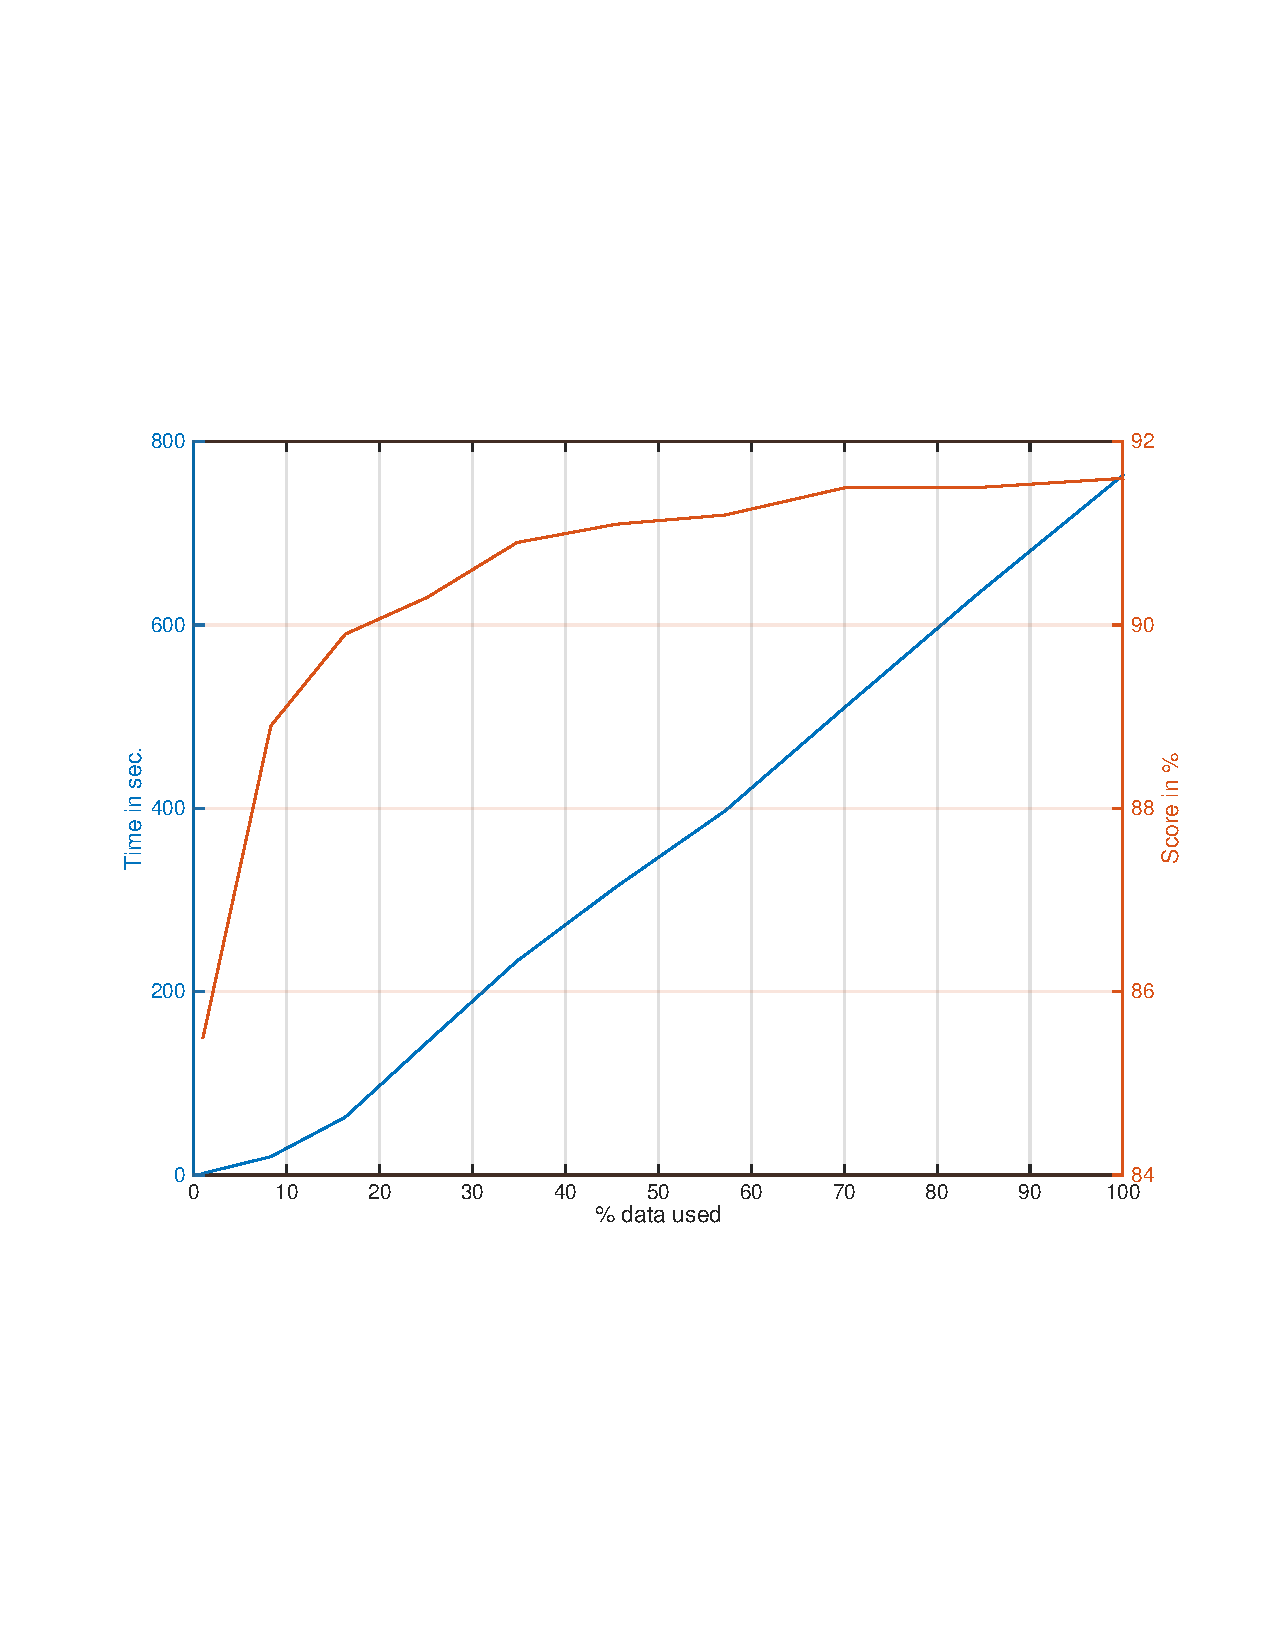
\includegraphics[trim=50 200 35 205,clip,width=.6\linewidth]{figures/lr_mnist.pdf}
  \caption{Running logistic regression on the MNIST dataset}
  \label{sampledata1}
\end{figure}

\begin{figure}
\centering
  \includegraphics[trim=50 200 35 205,clip,width=.6\linewidth]{figures/rf_mnist.pdf}
  \caption{Running random forest on the MNIST dataset}
  \label{sampledata2}
\end{figure}

% TODO maybe replace this with data/rnd-forest_mnist/
\begin{figure}
\centering
  \includegraphics[trim=50 200 35 205,clip,width=.6\linewidth]{figures/lr_synth.pdf}
  \caption{Running logistic regression on a synthetic dataset}
  \label{sampledata3}
\end{figure}

\begin{figure}
\centering
  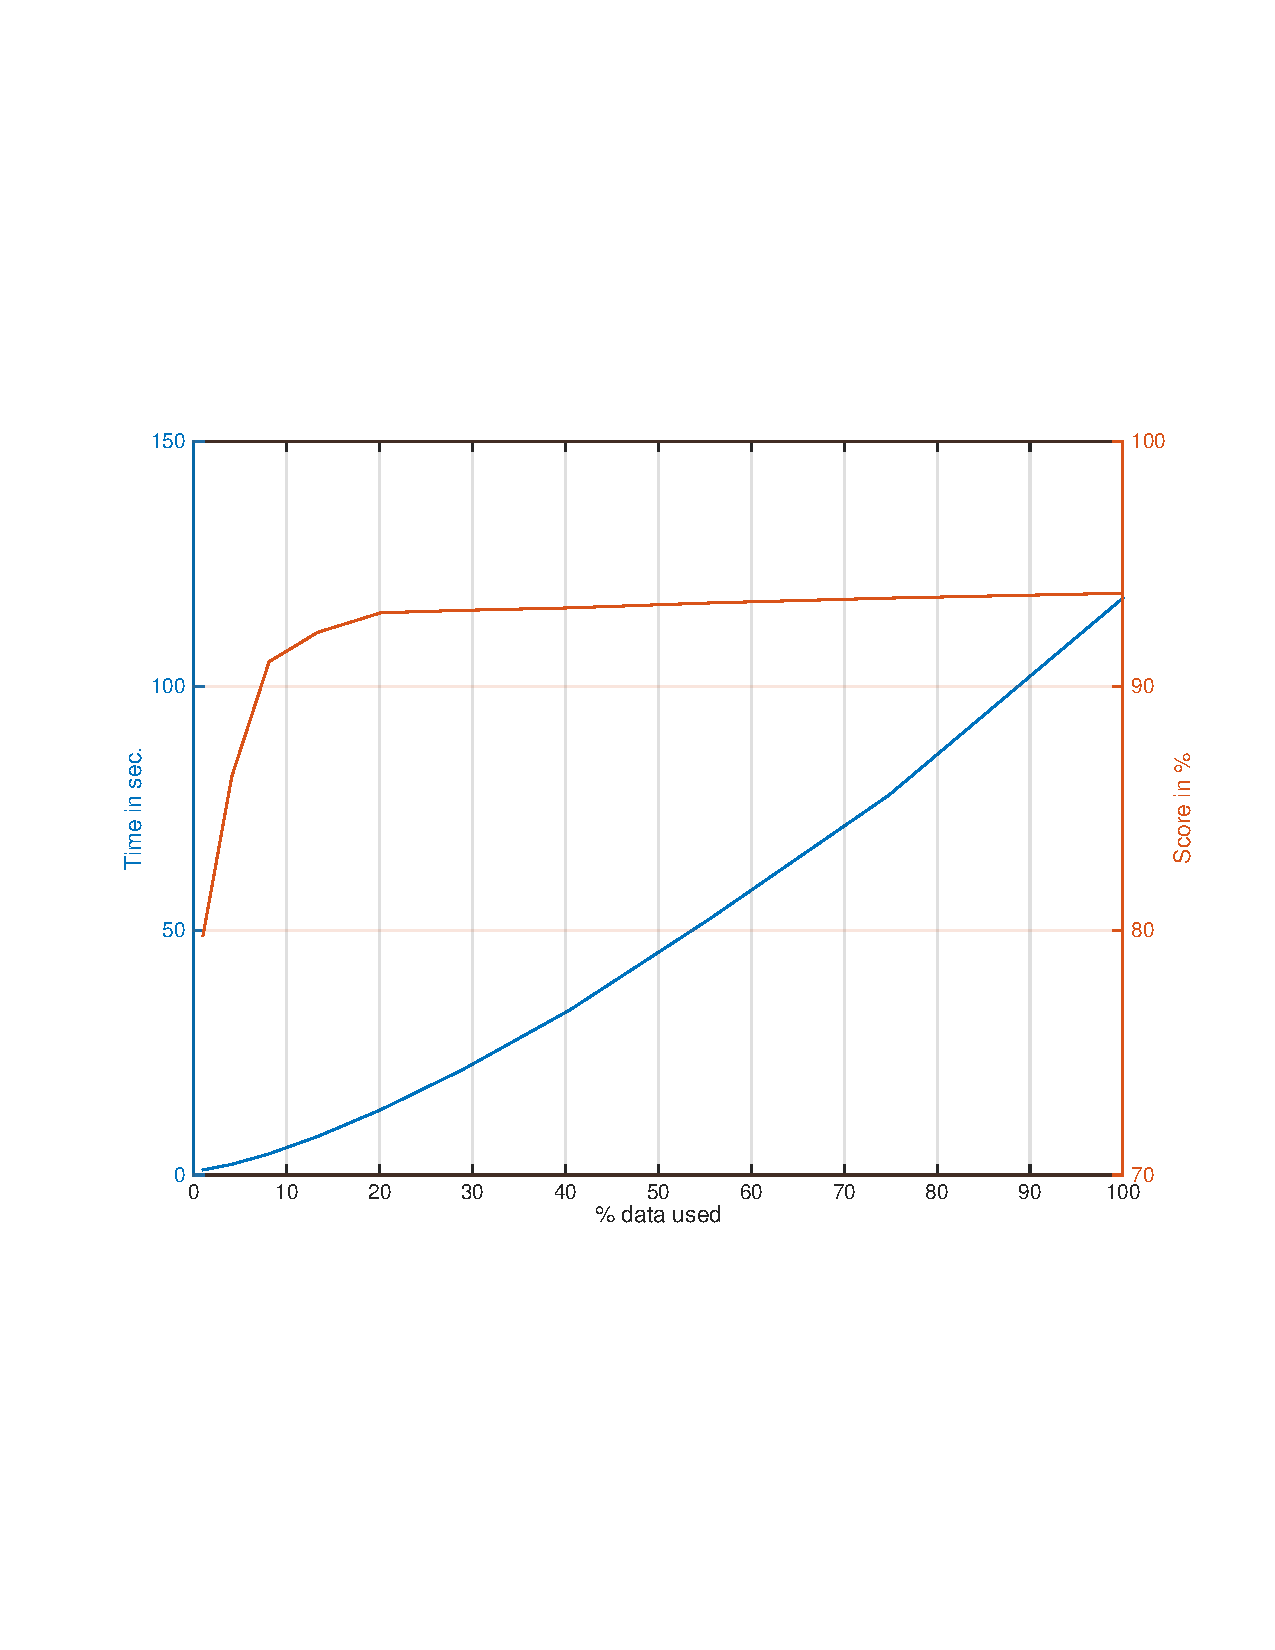
\includegraphics[trim=50 200 35 205,clip,width=.6\linewidth]{figures/rf_synth.pdf}
  \caption{Running random forest on a synthetic dataset}
  \label{sampledata4}
\end{figure}



% TODO why suddenly misclassification instead of accuracy, explain that one is 1-the other
Figures \ref{sampledata1}, \ref{sampledata2}, \ref{sampledata3} and \ref{sampledata4} show the results of collecting performance data, varying the percentage of data used. The four plots show the result of running random forest with 128 trees and logistic regression on the MNIST dataset and a synthetic dataset with 5000 samples and 500 features.

In all four figures, the run time shown in blue shows linear growth as the amount of data increases. As run time values shown in figure \ref{sampledata3} are substantially lower, the values are noisier than in the other graphs, which is to be expected. The run time shown in figure \ref{sampledata2} shows a change in growth at around 75\%. This is an effect which sometimes occurred during data collection and which we analyse in detail in the Challenges section of the Evaluation chapter.

The error rates for all four combinations of algorithms and datasets shown in red exhibits exponentially decaying behaviour, falling very rapidly initially before levelling off.

% TODO also show plot for # trees (or another appr param)








\section{The Exponential Mixture Kernel}
% TODO mention that this kernel is added to a linear kernel
% TODO change k to \kappa
% TODO use x, x' and t, t' consistently 

Based on the results shown in the previous section, we implemented a kernel to model the exponential behaviour of classification accuracy. Following \cite{2014arXiv1406.3896S}, we define the kernel as
% TODO JAMES can this be written as \psi(\lambda)d\lambda ?
\begin{align}
k(t,t') &= \int_{0}^{\infty} e^{-\lambda t}e^{-\lambda t'}\mu(d\lambda)\\
&= \int_{0}^{\infty} e^{-\lambda(t+t')}\mu(d\lambda)
\end{align}

% TODO kernel assumptions: decay starts at zero, maybe add limes
% TODO does this kernel always go to 0?
with $\mu$ being a mixing measure\footnote{We use $\mu$ instead of $\psi$ to denote the mixing measure to avoid confusion with the $\psi$ parameter to the gamma function explained below.}that weighs the $e^{-\lambda(t+t')}$ term. Note that this is not a stationary kernel as $k(t, t') \neq k(a + t, a + t')$. This conforms to our prior that moving further away from the origin, the value of $k$ should decrease.

Again following \cite{2014arXiv1406.3896S}, we choose a gamma distribution as $\mu$ which leads to an analytic solution to the integral:
\begin{align}
k(t, t') &= \int_0^{\infty} e^{-\lambda(t+t')}\frac{\beta^\alpha}{\Gamma(\alpha)}\lambda^{\alpha -1}e^{-\lambda\beta} d\lambda\\
&=\frac{\beta^\alpha}{\Gamma(\alpha)}\int_0^\infty e^{-\lambda(t+t'+\beta)}\lambda^{\alpha-1}d\lambda\\
&=\frac{\beta^\alpha}{(t+t'+\beta)^\alpha}
\end{align}

Diverging from \cite{2014arXiv1406.3896S}, we reparameterise the gamma distribution with
\begin{equation}
\psi = \mathbb{E}(x) = \frac{\alpha}{\beta}
\end{equation}
and
\begin{align}
\xi &= \frac{Var(x)}{\mathbb{E}^2 (x)} = \frac{\alpha}{\beta^2} \cdot \frac{\beta^2}{\alpha^2}\\
&= \frac{1}{\alpha}
\end{align}

\begin{figure}
\centering
\begin{subfigure}{.5\textwidth}
  \centering
  \includegraphics[trim=80 190 70 190,clip,width=0.95\linewidth]{figures/gamma_psi.pdf}
  \caption{Varying $\psi$, $\xi$ fixed at 1.1}
  \label{gammapsi}
\end{subfigure}%
\begin{subfigure}{.5\textwidth}
  \centering
  \includegraphics[trim=80 190 70 190,clip,width=0.95\linewidth]{figures/gamma_xi.pdf}
  \caption{Varying $\xi$, $\psi$ fixed at 1.1}
  \label{gammaxi}
\end{subfigure}
\caption{Varying the parameters to the reparameterised $\Gamma$-distribution}
\label{gammadist}
\end{figure}


Figure \ref{gammadist} show how the distribution changes as $\psi$ and $\xi$ are varied.
% TODO ADD how do they change
% TODO ADD say why this is convenient

After reparameterisation, the term for our kernel becomes
\begin{equation}
\kappa(x, x') = \frac{\frac{1}{\psi\xi}^{\frac{1}{\xi}}}{(x+x'+\frac{1}{\psi\xi})^{\frac{1}{\xi}}}
\end{equation}

\begin{figure}
\centering
\begin{subfigure}{.33\textwidth}
  \centering
  \includegraphics[trim=80 190 70 190,clip,width=\linewidth]{figures/expmix_psi1_xi1.pdf}
  \caption{$\psi=1$, $\xi=1$}
  \label{expmix11}
\end{subfigure}%
\begin{subfigure}{.33\textwidth}
  \centering
  \includegraphics[trim=80 190 70 190,clip,width=\linewidth]{figures/expmix_psi5_xi1.pdf}
  \caption{$\psi=5$, $\xi=1$}
  \label{expmix51}
\end{subfigure}%
\begin{subfigure}{.33\textwidth}
  \centering
  \includegraphics[trim=80 190 70 190,clip,width=\linewidth]{figures/expmix_psi10_xi1.pdf}
  \caption{$\psi=10$, $\xi=1$}
  \label{expmix101}
\end{subfigure}
\caption{Functions drawn from the kernel for three different values of $\psi$}
\label{kernelpsi}
\end{figure}

\begin{figure}
\centering
\begin{subfigure}{.33\textwidth}
  \centering
  \includegraphics[trim=80 190 70 190,clip,width=\linewidth]{figures/expmix_psi1_xi1.pdf}
  \caption{$\psi=1$, $\xi=1$}
  \label{expmix11_}
\end{subfigure}%
\begin{subfigure}{.33\textwidth}
  \centering
  \includegraphics[trim=80 190 70 190,clip,width=\linewidth]{figures/expmix_psi1_xi5.pdf}
  \caption{$\psi=1$, $\xi=5$}
  \label{expmix15}
\end{subfigure}%
\begin{subfigure}{.33\textwidth}
  \centering
  \includegraphics[trim=80 190 70 190,clip,width=\linewidth]{figures/expmix_psi1_xi10.pdf}
  \caption{$\psi=1$, $\xi=10$}
  \label{expmix110}
\end{subfigure}
\caption{Functions drawn from the kernel for three different values of $\xi$}
\label{kernelxi}
\end{figure}

Figures \ref{kernelpsi} and \ref{kernelxi} show the effect that varying $\psi$ and $\xi$ has on the kernel.

% TODO ADD iterpret these figures

The score functions shown in the previous section don't normally decay to zero, instead they plateau at values between zero and one. To model this effect, we add a constant function to our exponential mixture kernel as described in the Background chapter.

\section{Selecting Kernel Hyperparameters} 


To fit a Gaussian process to a given set of data points, one needs to find appropriate values for the hyperparameters to its covariance and likelihood function. There two main methods to achieve this are marginalisation and optimisation. For reasons explained in the evaluation chapter, we implement both of these methods in our project.

% TODO this algorithm is "too clever"
% TODO show figs where optimisation fails
GPML comes with an optimisation function that is meant to be used to optimise hyperparameters. It relies on gradient information which we implemented for the exponential mixture kernel. We were, however, not able to use this function with our kernel as it would terminate after a very small number of steps having barely moved from the initial values without having found a minimum. We suspect the reason for this to be numerical instability that creates very small local minima that the optimiser is unable to escape from. Figure @ shows an example of a marginal likelihood function that we tried to optimise with GPML's \texttt{minimize}.

After failing to optimise the hyperparameters to our kernel using the optimisation function included with GPML, we decided to implement sampling which does not suffer from the same problems as optimisation. For reasons of speed and ease of use, we then decided to implement our own optimisation routine which is described in detail below. An evaluation of the two methods applied to our data can be found in the Evaluation chapter.


\subsection{Sampling}
The first approach to hyperparameter selection we use in our project is the Bayesian approach of integrating out the hyperparameters $\theta$:

% TODO maybe murphy equation 15.1
\begin{equation}
p(y|X) = \int p(y|X,\theta)p(\theta)d\theta\\
\end{equation}

We decided to implement slice sampling
decided to implement this when gpml minimise didn't work

The main advantage of sampling the hyperparameters is that it does not suffer from overfitting the same way optimisation does, given that the samples are successfully drawn from the posterior distribution. Its major drawback is that it is computationally more expensive than optimisation methods. Implementation wise, sampling also takes more effort than optimisation, as the result of the computations the program executes have to be correctly averaged over.

% integral has no analytic solution -> approximated with MCMC -> what's mcmc -> we use slice sampling

% TODO ADD finish this

%The Bayesian way to handle hyperparameters is to integrate them out. 
% TODO add maths on integrating out hyperparams

%To approximate this integral, MCMC methods are
% TODO maths on MCMC

%To sample from @ we use slice sampling. adv/disadv: \cite{neal2003}
% TODO why slice sampling and not another method
%- mcmc/sampling



\subsection{Optimisation}
Another approach to find suitable hyperparameters is to optimise the marginal likelihood of the model with respect to its hyperparameters. This has the advantage of being substantially faster than sampling. It is also easier to implement, as it returns one set of hyperparameters that can be used to make predictions instead of multiple samples that have to be correctly averaged over.

The great disadvantage of optimisation is that it is prone to overfitting by choosing one optimum in cases where multiple viable optima exist. We describe situations in which we encountered this problem in the Evaluation chapter, comparing it with the results of slice sampling.



After inspecting the marginal likelihood function @of sample data@ in Matlab, we concluded that it is not a function that is inherently difficult to optimise and decided to implement our own optimisation routine. As we had already successfully sampled hyperparameters using slice sampling as described above, we implemented an optimisation method that works similarly to how slice sampling draws samples. The first version of this algorithm is shown below as Algorithm \ref{opti1}.


\begin{algorithm}
\begin{algorithmic}[1]
\Procedure{Slice\_optimisation}{$f,x,iterations=100,width=1$}
\State $y\gets f(x),\ D\gets \Call{get\_dimensions}{x}$
\For{$i\gets 1, iterations$}
\For{$dim\gets \Call{permute}{D}$}\Comment{Iterate over all dimensions}
\State $x_l, x_r, x'\gets x$\Comment{$x_l,\ x_r$ span interval, $x'$ falls inside}
\State $r\gets \Call{Uniform}{0, 1}$
\State $x_l(dim)\gets x(dim) - r * width$
\State $x_r(dim)\gets x(dim) + (1 - r) * width$
\For{$j\gets 1, 15$}
\State $x'(dim)\gets \Call{Uniform}{x_r(dim), x_l(dim)}$
\State $y' = f(x')$
\If{$y' < y$}
\State $y\gets y',\ x(dim) = x'(dim)$\Comment{New optimum}
\Break
\EndIf
\If{$x'(dim) > x(dim)$}
\State $x_r(dim) = x'(dim)$\Comment{Narrow interval from the right}
\ElsIf{$x'(dim < x(dim)$}
\State $x_l(dim) = x'(dim)$\Comment{Narrow interval from the left}
\EndIf
\EndFor
\EndFor
\EndFor
\EndProcedure
\end{algorithmic}
\caption{First version of slice optimisation}
\label{opti1}
\end{algorithm}

This optimisation algorithm starts at a given $x$ and optimises by iterating over the input dimensions, spanning up an interval around $x$ for every iteration. Inside of these iterations, it selects points $x'$ at random from the interval. If $f(x')$ is smaller than the current minimum, it continues to the next loop iteration, otherwise it narrows the interval either from the left or the right, depending on the side of $x$ on which $x'$ falls.

Given enough data, this algorithm is able to find suitable hyperparameters to the exponential mixture kernel reliably. If it is used to fit a GP to a small number of points (five or less), it often selects hyperparameters such that the covariance matrix is not positive semidefinite and Cholesky decomposition fails. We catch these errors by wrapping every evaluation of $f$ in a \texttt{try ... catch} block. 

While testing this algorithm, we found an effective method to handle these errors to be rerunning the algorithm multiple times and selecting the result with the highest marginal likelihood. This also alleviates the issue of local optima which we discuss in detail in the Evaluation chapter. The code to achieve this is shown as Algorithm \ref{optiwrap}.

\begin{algorithm}
\begin{algorithmic}[1]
\Procedure{Optimise\_with\_restarts}{$f,x,restarts=5$}
\State $X = [\ ],\ Y = [\ ]$
\For{$i\gets 1, restarts$}
\State $x'\gets \Call{Slice\_optimisation}{f, x}$
\State $y'\gets f(x')$
\State $\Call{append}{X, x'}$
\State $\Call{append}{Y, y'}$
\EndFor
\State $i\gets \Call{MinIndex}{Y}$
\State \textbf{return} $X(i)$
\EndProcedure
\end{algorithmic}
\caption{Rerunning the optimiser}
\label{optiwrap}
\end{algorithm}

% TODO stress that this is only important for development and that when using actual data, this would get dominated (in the evaluation chapter)
While this updated algorithm produces adequate results, it takes a substantial amount of time to optimise. A final change we therefore added was to terminate the optimisation routine early if the value of $y$ only changes minimally between five optimisations. This condition is met during almost all iterations and often drastically cuts short the time that our algorithm needs.

% TODO MAYBE mention that there is an implementation of it, what did you try to make it work?
One shortcoming of this optimisation routine is that all its steps have to be axis aligned. If the gradient of the function being optimised at $x$ is not aligned with any axis, this causes the optimiser to make very small steps along multiple axes. A superior approach would be to directly move along the gradients, which are available to us. As our current algorithm already performs to a high standard, we did not investigate this potential improvement further.


% TODO mention that the result of optimisation is handled as one sample, averaged over one


%show diagrams, talk about the relationship. is it always linear for time (no, svm, O(n^2-3)), is it always exponential for score

% TODO move this to evaluation
\subsection{Using both methods} % TODO different name

As our program has to be able to handle both samples and single results returned by optimisation, we decided to treat the result of our optimisation routine as a single sample in the routines that make use of our model. This makes it completely transparent to these routines which of the two hyperparameter selection methods were used and enables us to switch between them according to the requirements of the schedulers.

% TODO END hyperparameter spelling

% TODO END go over all section/chapter headings again
% TODO END "classification accuracy" maybe isn't correct if we also use roc
% TODO END mention somewhere that "performance" means time + score
% TODO END sort out use of "classification accuracy", "accuracy", "performance", "score"
\chapter{Scheduling} 



\textit{This chapter describes the theoretical and practical aspects system we developed. It firsts gives a high level overview of the system architecture before describing in detail how the scheduling heuristics used try to to find optima within the time constraints.}

\section{System Architecture}
\subsection{High level architecture}
\begin{figure}[p]
    \centerline{\includegraphics[trim=40 90 35 90,clip,scale=0.8]{figures/architecture3.pdf}}
  \caption{High level architecture for one scheduler, shown after three iterations. Data is shown in green, machine learning algorithm in red and the scheduler in blue. Circled numbers refer to notes in the text.}
    \label{architecture}
\end{figure}

% TODO 2d kernel

% TODO say in the beginning that we focus on rndforest/log reg and % data
Our system is designed in a two tiered fashion. Tier 1 creates models of the data using learning algorithms that are parameterised with approximation parameters. The training time and accuracy of these models makes up the input to tier 2. This second layer first creates meta-models of the running time and score of the models in tier 1. These meta-models are then used by the scheduler to select the algorithm and approximation parameters for the next iteration and the process is repeated.

In this system, we focus on the two algorithms described in the background chapter

Figure \ref{architecture} shows this architecture diagrammatically for one scheduler after three iterations. In tier 1, the dataset (1) is used as input to all learning. The learning process is parameterised by the learning algorithm and the approximation parameters to the algorithm (2). The running time and score for every iteration are saved (3) separately for every array. This saved data is then. 

In tier 2, this performance data is used to train two Gaussian process, a linear one for the time and one based on the exponential mixture kernel for the score (4). The models 

% TODO ADD finish this

%Note how both tiers execute machine learning algorithms on data (coloured in green) and how the result of the algorithms in the first tier form the data set for the Gaussian Process at the top of the diagram. The main loop of our program is shown, slightly simplified, in Figure \ref{mainloop}. When executing, the program switches back and forth between the two tiers: it executes an algorithm with a given set of approximation parameters, builds a new model that includes the performance during this execution. The scheduler then decides which algorithm/approximation parameter combination to run next and the system returns to the first step.

% TODO explain how every scheduler optimises over multiple algorithms, each algorithm has its own acquisition function
% TODO four vectors: score m/sd, time m/sd
% TODO explain burn in better and how you don't model during burn in
% TODO mention drawing
% TODO mention how multiple schedulers can be executed simultaneously
% TODO mention that schedulers have aqcuisition function
% TODO mention time limit threshold
% TODO include and explain figure  of two schedulers running at the same time, also show sampling
% TODO go more into details of what schedulers do
% TODO mention that all the performances are recorded and new datapoints are appended

\begin{figure}[ht]
\begin{lstlisting}[language=Python]
while True:
   scheduler.decide() # Tier 2 (scheduling)
   if scheduler.decision:
      scheduler.execute() # Tier 1
      scheduler.model() # Tier 2 (modelling)
\end{lstlisting}
\caption{The main loop}
\label{mainloop}
\end{figure}


\subsection{Directory structure of the code}

The directory of the project contains the following subdirectories:
\begin{itemize}
\item \textbf{data/}: This directory contains datasets in \texttt{data/raw\_arffs/}. It is also where data generated by the data generation scripts are stored. When creating plots based on this data, the results are written into this folder
\item \textbf{figs/}: Every diagram that our system generates is automatically also saved to this directory
\item \textbf{report}/: This folder is where the source file and diagrams for this document are stored
\item \textbf{src/}: This directory holds all the source code for our project. It contains \texttt{main.py}, the main code file and two subdirectories, \texttt{src/data\_handling/} and \texttt{src/matlab/} which contain Python and Matlab code respectively
\item \textbf{var/}: This folder is used to store temporary files that are used to exchange data between Python and Matlab code
\end{itemize}

\subsection{Interoperability between Python and Matlab}
Choosing Matlab to implement the performance modelling code and Python to implement the other parts of our system made it necessary to devise a method of transferring data between these two parts of the program. During the initial planning stage, we intended to write all parts of the system in Python but the advantages of GPML such as level of documentation and ease of use later turned out to outweigh the disadvantages of dealing with process interoperability.

To start the program, the \texttt{main.py} file is executed. This file then periodically calls a Matlab script whenever it has collected new data and needs to update one of its performance models. Data is transferred between the Python and the Matlab scripts by writing it to \texttt{json} files\footnote{JSON is a widespread data format similar to XML.}. Before this script is executed, \texttt{main.py} writes the recorded performances of the algorithm for which it has just updated its data to \texttt{var/scheduler\_data.json}. This file contains a JSON object with the fields \texttt{x\_percent\_data}, \texttt{y\_times} and \texttt{y\_scores} which hold the data collected so far.

Once it has finished modelling, the Matlab script writes the models to \texttt{var/models.json} and terminates. This file contains an array of model objects. These models are represented as 100 equally spaced data points between 0 and 100 \%. They each have an \texttt{m} and an \texttt{sd} field set for mean and standard deviation respectively. This file is then read by \texttt{main.py} and the old models are overwritten with the updated values.


% TODO move this up to the prev chapter
\section{Measuring performance}
% TODO END Cross-Validation spelling
As shown in figure \ref{architecture}, the output of tier 1 is the performance of the model that the learning algorithm creates of the dataset given the particular approximation parameters that are selected by the scheduler. This section explains how the performance of the models is measured. Specifically, we describe how we measure predictive accuracy and training time of our models.

\subsection{Classification accuracy}

Measuring classification accuracy is more complex than stopping time. One common approach to measure the performance of a model is to split the dataset into two subsets, train the model on one subset and compare its predictions on the second subset with the actual values. This method has the disadvantage that only a subset of the available data is used for training which can make it susceptible to variance in reported classification accuracy depending on how the data is split.

A superior method, that we slightly adjust to the requirements of this project is k-Fold Cross-Validation. This approach to measure model performance splits the dataset into $k$ subsets of equal size, here called folds. The algorithm then learns on the combined data of the second to $k$th folds, using the first fold as a validation set. This process is repeated $k$-times, using another fold as validation set in each iteration. The classification accuracies of the $k$ iterations are then averaged to calculate the overall classification accuracy. This approach ensures that all the data is used for training. Although the learning algorithm has to be executed $k$ times instead of just one, $k$ is a constant value in k-Fold Cross-Validation that does not depend on the size of the dataset and therefore does not impact the asymptotic run time.

To implement the percentage of data approximation parameter, we need to restrict the data that is used for training our models while still keeping the advantages of k-fold cross-validation. We achieve this by further splitting the folds used for training. For each fold, a subset of samples is selected according to the percentage of data to be used. The fold used for validation, however, does not change. This approach ensures that all available data is used for validation.

The classification accuracy in cases where the samples belong to more than one class is calculated as the percentage of samples whose class was correctly predicted. Using two different scoring algorithms is valid because we never compare performance across datasets.

% TODO add diagram, give better intuition
When calculating the score that a model achieves on a given validation set, two different methods are used. For binary classification tasks\footnote{Those in which each sample belongs to one of two classes such as \texttt{true} and \texttt{false}.}, we use the receiver operating characteristic (ROC) metric to asses model accuracy. This metric calculates the percentage of the area under the curve that plots the false positive rate of the classifier against its true positive rate. This metric has been shown to be more robust than the simpler accuracy metric we use in the multiclass case \cite{Bradley97theuse}. Calculating an ROC curve is only possible for binary classification tasks because true and false positive rates are not defined in this case.

\subsection{Time}
Measuring the time spent learning is more straightforward than measuring classification accuracy. We use Python's \texttt{time.time()} function to stop the time that elapses while training. As we don't want to include validation time spent in the iterations of Cross-Validation, we keep the current time spent in a variable that gets updated after training in each iteration finishes.

Another factor to be considered is that other tasks running in parallel can pollute the timing data. During development of the program, we were on occasion forced to shut down resource intensive programs while running tests. This problem did not occur on the EC2 instance. % TODO why not?


% TODO explain why this doesn't underestimate performance by not using all the data

Before we split the dataset into the ten folds, we shuffle the samples to ensure proper randomisation across the folds. 






% TODO END don't just use "algorithms", use learning algorithms. also "performance model", not just "model"







\section{Implemented Schedulers}
% TODO JAMES add code to this?

Every scheduler is implemented in a separate class of which there are nine in total. There are three abstract scheduler classes that implement functionality shared between two or more schedulers while the other six implement scheduling strategies that can be used to schedule data collection. In this section, we describe each scheduler's functionality before comparing and evaluating them in the Evaluation chapter.

\subsection{\texttt{\textit{Scheduler}}}
This is the base class that all schedulers inherit from. It defines a framework general enough that all schedulers implement it. Besides drawing routines, which are mostly shared among schedulers, and code to write performance data and read model data, this class contains the following methods:

\begin{itemize}
\item \texttt{\_\_init\_\_}: the class constructer initialises a number of properties, including the \texttt{self.data} property which holds an array of learning performances for each algorithm
\item \texttt{decide}: this is a virtual method that is called to decide on the next algorithm/approximation parameter combination to be evaluated. It sets the \texttt{self.decision} property of the scheduler object. If the scheduler is done, either due to having finished optimising or because its time budget has been used up, this property is set to \texttt{None}
\item \texttt{execute}: this method executes the decision made by the \texttt{decide} method and adds the new time and score to the \texttt{self.data} property
\item \texttt{model}: this function updates the model for the algorithm for which data was collected during the last execution of the \texttt{execute} method. It reads the value of the \texttt{self.decision} property to determine the algorithm and is to be called after \texttt{execute} finishes
\end{itemize}


\subsection{\texttt{FixedSequenceScheduler}}
\texttt{FixedSequenceScheduler} is the simplest of all the scheduling strategies implemented. Its constructor takes a sequence of data percentage values and computes the cartesian product of the learning algorithms and this sequence and saves this list. When its \texttt{decide} method is called, it writes the next element of the list into \texttt{self.decision}, cycling through algorithms and executing the fixed sequence of data percentage values. Once it has executed every algorithm/data percentage, this scheduler terminates.

This scheduler is unique among the schedulers in not requiring the time and score to be modelled. Its evaluation sequence is set at initialisation and it does not rely on predictions to decide which learning algorithm/approximation parameter combination to try next.



\subsection{\texttt{\textit{ProbablisticScheduler}}}
This is a base class of all schedulers that make probabilistic decisions using an acquisition function as described in the Bayesian optimisation section in the Background chapter. It has a virtual class method \texttt{a} that takes a time and score model (expressed as arrays of mean and standard deviation) and calculates the acquisition function as array.

If slice sampling was used to integrate out the hyperparameters to the exponential mixture kernel, \texttt{\textit{ProbablisticScheduler}} is responsible for calling \texttt{a} as many times as there are samples and averaging over these acquisition functions. Time and score model samples are taken independently which allows us to randomly pair one time and one score model per iteration.

\subsection{\texttt{ProbabilityOfImprovementScheduler}}
This is the simplest concrete probabilistic scheduler. It implements the probability of improvement heuristic for Bayesian optimisation. As mentioned in the background chapter, this is not a competitive scheduling strategy but is still included for purposes of comparison.

This scheduler truncates its acquisition function at the maximum x value for each algorithm and only considers percentage of data values that are strictly greater than its current maximum. This encodes the assumption that using more data can never be worse than the current best result.

Figure @ shows the \texttt{ProbabilityOfImprovementScheduler} after a few iterations. Note how its acquisition function quickly drops off as uncertainty grows.

\subsection{\texttt{ExpectedImprovementScheduler}}
\texttt{ExpectedImprovementScheduler} implements the Expected improvement heuristics for Bayesian optimisation. Like the \texttt{ProbabilityOfImprovementScheduler}, it truncates its acquisition function and only considers using more data than before for subsequent execution of the learning algorithms.

\subsection{\texttt{ExpectedImprovementPerTimeScheduler}}
This scheduler inherits from the \texttt{ExpectedImprovementScheduler} and differs from it only by dividing the expected improvement by the mean of the time model. This biases it towards faster executions of the learning algorithms, even if the improvement over the current best is not as large as slower executions.

\subsection{\texttt{\textit{TimedScheduler}}}
\texttt{\textit{TimedScheduler}} is a superclass of the two schedulers that base their scheduling decisions on having a finite time budget. It inherits from \texttt{\textit{ProbablisticScheduler}} and includes functionality to keep track of the remaining time and add a line to the time plot to show how much time is left.

\subsection{\texttt{ExpectedImprovementTimesProbOfSuccessScheduler}}
This scheduler inherits from both the \texttt{\textit{TimedScheduler}} and the \texttt{ExpectedImprovementScheduler}. To compute its acquisition function, it multiplies the expected improvement with the probability of successfully finishing the learning process in the remaining time. The probability of success is calculated by cutting off the distributions of the time model at each point on the x-axis and computing the amount of probability mass under that point.

The constructor of \texttt{ExpectedImprovementTimesProbOfSuccessScheduler} expects a sequence of time intervals. Whenever the scheduler has used up its available time budget, the time interval in the sequence is added to the remaining time. % TODO give an example

\subsection{\texttt{MinimeseUncertaintyThenExploitScheduler}}
The \texttt{MinimeseUncertaintyThenExploitScheduler} inherits from \texttt{\textit{TimedScheduler}}. It has two scheduling phases and is allocated a time budget for each phase. Initially, it tries to understand the function and reduce uncertainty about its shape. Its acquisition is calculated as the uncertainty about the score, divided by the time it takes to evaluate the function at the point under consideration. This behaviour is similar to the \texttt{ExpectedImprovementPerTimeScheduler}.

After using up the time allotted for exploration, this scheduler uses the second time budget to construct the best model it can within that time, using the understanding of the function it gained during the first phase.

% TODO JAMES figures of strategies in this chapter or in evaluation?
% TODO mention somewhere that a resolution of 100 points is used



\chapter{Evaluation}
% TODO point cloud/graph that shows that one is better at first, then the other (for data vs score and time vs score)
\textit{This chapter describes the results that our system achieved. It also lists challenges that we faced during its development and limitations it currently has.}

% TODO PROGRAM skewed datasets with lots of pos, few neg

% TODO hinge: show plots where it occurs early and has little impact on modelling

% TODO evaluate kernel (model evidence etc)
% TODO for 2d: plot variance
 
% TODO optimisation is faster and produces only one mean/sd, easier to use
% using the \texttt{checkgrad.m}
% compare optimisation/sampling adv/disadv
% TODO rasmussen: local maxima correspond to a particular interpretation of the data

% TODO describe characteristics of all schedulers



\section{Data sources}
The second source of datasets we used was created synthetically using scikit-learn's \texttt{make\_classification} function. This function takes a number of parameters that define the dataset, such as the number of samples, the number of features and the number of classes and creates data according to these parameters. 

The fine grained control over the datasets that this function allows was very valuable to us, as it allowed us to see how our system handles datasets of different nature. We wrote a small script to enable us to quickly create datasets and see how logistic regression and random forest perform on subsets of these datasets.

% TODO actually mention this
A second source of datasets were drawn from the list of datasets that were used in the development of Auto-WEKA as mentioned in the Related Work chapter. The authors of Auto-WEKA made the datasets used to test Auto-WEKA available on their website\footnote{They can be downloaded at http://www.cs.ubc.ca/labs/beta/Projects/autoweka/datasets/}.

These datasets originally came from other sources \cite{Lichman:2013, Larochelle:2007:EED:1273496.1273556, Krizhevsky09learningmultiple} and were converted by the Auto-WEKA creators to WEKA's own dataformat, the Attribute-Relation File Format (\texttt{arff}). This made it very convenient for us to use these datasets as they are originally in a wide range of differing data formats and would have had to have individual import routines written for them. 

Besides converting them to the \texttt{arff} format, the authors of the Auto-WEKA paper also split them up in a training and a test set. As we described in the Implementation chapter, we immplement k-fold-cross-validation and therefore needed all the data in a single set. To achieve this, a small ruby script was written to merge the \texttt{train.arff} and \texttt{test.arff} files for each dataset.

% TODO show table with size (MB), #features, #samples, #classes

While some of the datasets in this collection are entirely numerical, some have textual features while still others have a mixture of strings and numbers as features. An example of this is the \texttt{germancredit} dataset which has a feature \texttt{credit\_history} with possible values such as \texttt{"all paid"} and \texttt{"critical/other existing credit"} and a feature,  \texttt{age}, which is a number.

When using these datasets, we load the \texttt{arff} files using SciPy's \texttt{scipy.io.arff.loadarff} function. As scikit-learn expects the features to all be numerical, we convert the data using a one-of-k encoding.

% TODO kein konjunktiv
This encoding expands every feature of type string with $n$ possible values into $n$ boolean typed features. This means that a feature such as \texttt{other\_payment\_plans}, also taken from the \texttt{germancredit} dataset, with possible values \texttt{bank}, \texttt{stores} and \texttt{none} would be converted to three separate features, \texttt{other\_payment\_plans=bank}, \texttt{other\_payment\_plans=stores} and \texttt{other\_payment\_plans=none}. For every sample in the dataset, one of these features would be set to $1$ and all others to $0$

Another issue we faced when using the Auto-WEKA datasets is that the \texttt{arff} file format allows are sparse encoding for datasets that mostly contain zeros. Other datasets contain samples with missing values. SciPy's \texttt{loadarff} routine is not currently able to open either of these two types of \texttt{arff} files these files.

% TODO explain why this is not a problem: we select datasets already b/c the small ones are too small to further increase data; the interesting ones work?

% TODO END maybe always distinguish between model and meta-model
\section{Model comparison}
% TODO ADD finish this section

% artificial data
% TODO marginal likelihood
% TODO how much variance gets explained
% TODO show and discuss plots

\section{The Exponential Mixture Kernel}




\subsection{Hyperparameter selection}
We generally found both of the methods we use for hyperparameter selection, sampling and optimisation, to return satisfying results. As is in the nature of optimisation, however, it is prone to overfit. This is an issue especially in the early phases of data collection after a few iterations when only little data was available.
% TODO show figure

One way we addressed this problem was by increasing the number of data points collected during the burn in phase. As the subsets used in this phase are a small percentage of the whole dataset, this only adds marginally to the time that is spent on burn-in.

% TODO is this really true? verify
Although this addressed the issue of overfitting on too little data, sampling hyperparameters still proved more robust and less likely to return models that clash with the expectations that we had looking at the data.


%\subsection{Unexpected behaviour}
% TODO MAYBE mention kernel "cliffs"


\section{Scheduling Results}
% TODO finish this section

% TODO show case where one function is better initially but then gets overtaken

\subsection{Scheduler Behaviour}


\subsubsection{\texttt{FixedSequenceScheduler}}
\begin{figure}
\centering
% TODO FIGURE trim this to only show fixed sequence scheduler
  \includegraphics[trim=0 0 0 0,clip,width=\textwidth]{figures/fixed_sequence_example.pdf}
  \caption{A fixed exponential sequence}
  \label{fixedsequenceexample}
\end{figure}

Figure \ref{fixedsequenceexample} shows a \texttt{FixedSequenceScheduler} with a geometric sequence of data percentage values after a number of iterations. In the last iteration, it trained logistic regression with about 80\% of the available data (the rightmost blue dot on both subplots) and is about to learn using random forests on the same amount of data.

This scheduler does not model performance data and does not adjust its decisions during the course of its execution.

% TODO END explain and distinguish score, performance, accuracy, time, error early on
% TODO explain how there are multiple acquisition functions, maximum of all of them is selected

\subsubsection{\texttt{ProbabilityOfImprovementScheduler}}
\begin{figure}
\centering
% TODO FIGURE trim this to only show fixed sequence scheduler
  \includegraphics[trim=530 495 510 295,clip,width=\textwidth]{figures/prob_of_imp_01.pdf}
  \caption{Probability of improvement acquisition function}
  \label{sched:probofimpr1}
\end{figure}

The \texttt{ProbabilityOfImprovementScheduler} tends to be conservative in exploring the function. Figure \ref{sched:probofimpr1} shows the score models and the acquisition functions for both algorithms as dashed lines. Although it models the blue algorithm to have a higher score for all $x$ values, it is less sure about how the score of this algorithm changes as $x$ grows. Consequently, it will evaluate the red algorithm next.

Although the uncertainty about the performance of the red algorithm does not change much for larger x values, as it does for the blue algorithm, the probability of improvement acquisition function for the red algorithm has its maximum at about 0.25 and decreases for larger values than that. This is due to the fact that the probability of improvement scheduler does not consider the magnitude of the increase over the current best value.

\begin{figure}
\centering
% TODO FIGURE trim this to only show fixed sequence scheduler
  \includegraphics[trim=530 270 507 510,clip,width=\textwidth]{figures/prob_of_imp_02.pdf}
  \caption{Probability of improvement acquisition function}
  \label{sched:probofimpr2}
\end{figure}

Figure \ref{sched:probofimpr2} shows a situation similar to the one shown in figure \ref{sched:probofimpr1} with the difference that the uncertainty is roughly equal for both algorithms. The acquisition functions behave accordingly with the acquisition function for the red algorithm being lower because it is less likely to improve over the current maximum $y$ which was achieved by the blue algorithm.

\begin{figure}
\centering
% TODO FIGURE trim this to only show fixed sequence scheduler
  \includegraphics[trim=530 710 493 55,clip,width=\textwidth]{figures/prob_of_imp_03.pdf}
  \caption{Probability of improvement acquisition function}
  \label{sched:probofimpr3}
\end{figure}

In figure \ref{sched:probofimpr3}, we see the final state of a probability of improvement scheduler. The small step size for evaluating the blue algorithm is a typical behaviour of this scheduler. 

\subsubsection{\texttt{ExpectedImprovementScheduler}}

Although the purpose of this scheduler in our program is to function as a superclass for more complex schedulers, it is nevertheless necessary to study its behaviour to understand these later schedulers.

% TODO make sure to mention exploration/exploitation trade-off when explaining EI above, maybe show integral here, rewrite this to make sure it's correct.
Figure \ref{sched:expimpr01} shows typical acquisition functions for the \texttt{ExpectedImprovementScheduler}. Recall that the expected improvement strategy automatically balances exploration and exploitation, and that both, a high mean and a high variance increase the value of the acquisition function. Figure \ref{sched:expimpr01} demonstrates this effect: while the mean for the blue and the red algorithms for x values greater than about 0.4 are almost equal, the expected improvement for the red algorithm overtakes the one for the blue algorithm because its variance is greater.

\begin{figure}
\centering
% TODO FIGURE trim this to only show fixed sequence scheduler
  \includegraphics[trim=530 710 493 55,clip,width=\textwidth]{figures/expimpr01.pdf}
  \caption{Expected improvement acquisition function}
  \label{sched:expimpr01}
\end{figure}



\subsubsection{\texttt{ExpectedImprovementPerTimeScheduler}}
\begin{figure}
\centering
% TODO FIGURE trim this to only show fixed sequence scheduler
  \includegraphics[trim=140 710 493 55,clip,width=\textwidth]{figures/ei_by_time_1.pdf}
  \caption{Expected improvement per time performance models and acquisition function}
  \label{sched:expimprpertime01}
\end{figure}

The \texttt{ExpectedImprovementPerTimeScheduler} is a slight variation of the \texttt{ExpectedImprovementScheduler}. To calculate its acquisition function, it divides the expected improvement by the mean of the time model. Figure \ref{sched:expimprpertime01} shows the bias this scheduler has towards function evaluations that are predicted to be fast. Although the expected improvement increases as shown in figure label{sched:expimpr01}, the required time also grows (shown on the left).

% TODO in the scheduler explanation section, mention that "success" means finishing in time
% TODO emphasize that these are the two truly new schedulers, anytime & contract
% TODO mention that some schedulers trim their acquisition functions while others dont
\subsubsection{\texttt{ExpectedImprovementTimesProbOfSuccessScheduler}}
% TODO say what this scheduler is for (anytime)

This is one of the two schedulers that expect to be given a time budget during initialisation. Figure \ref{sched:expimprpertime01} shows the state of the scheduler after the burn in phase having been alloted one second to spend. This time limit is marked on the left plot. As can be seen on that plot, the probability that evaluating the red algorithm with an x value higher than the current maximum of 0.15 will finish in time is extremely low. Consequently, the acquisition function for the red algorithm is essentially flat and not visible in the right plot.

\begin{figure}
\centering
  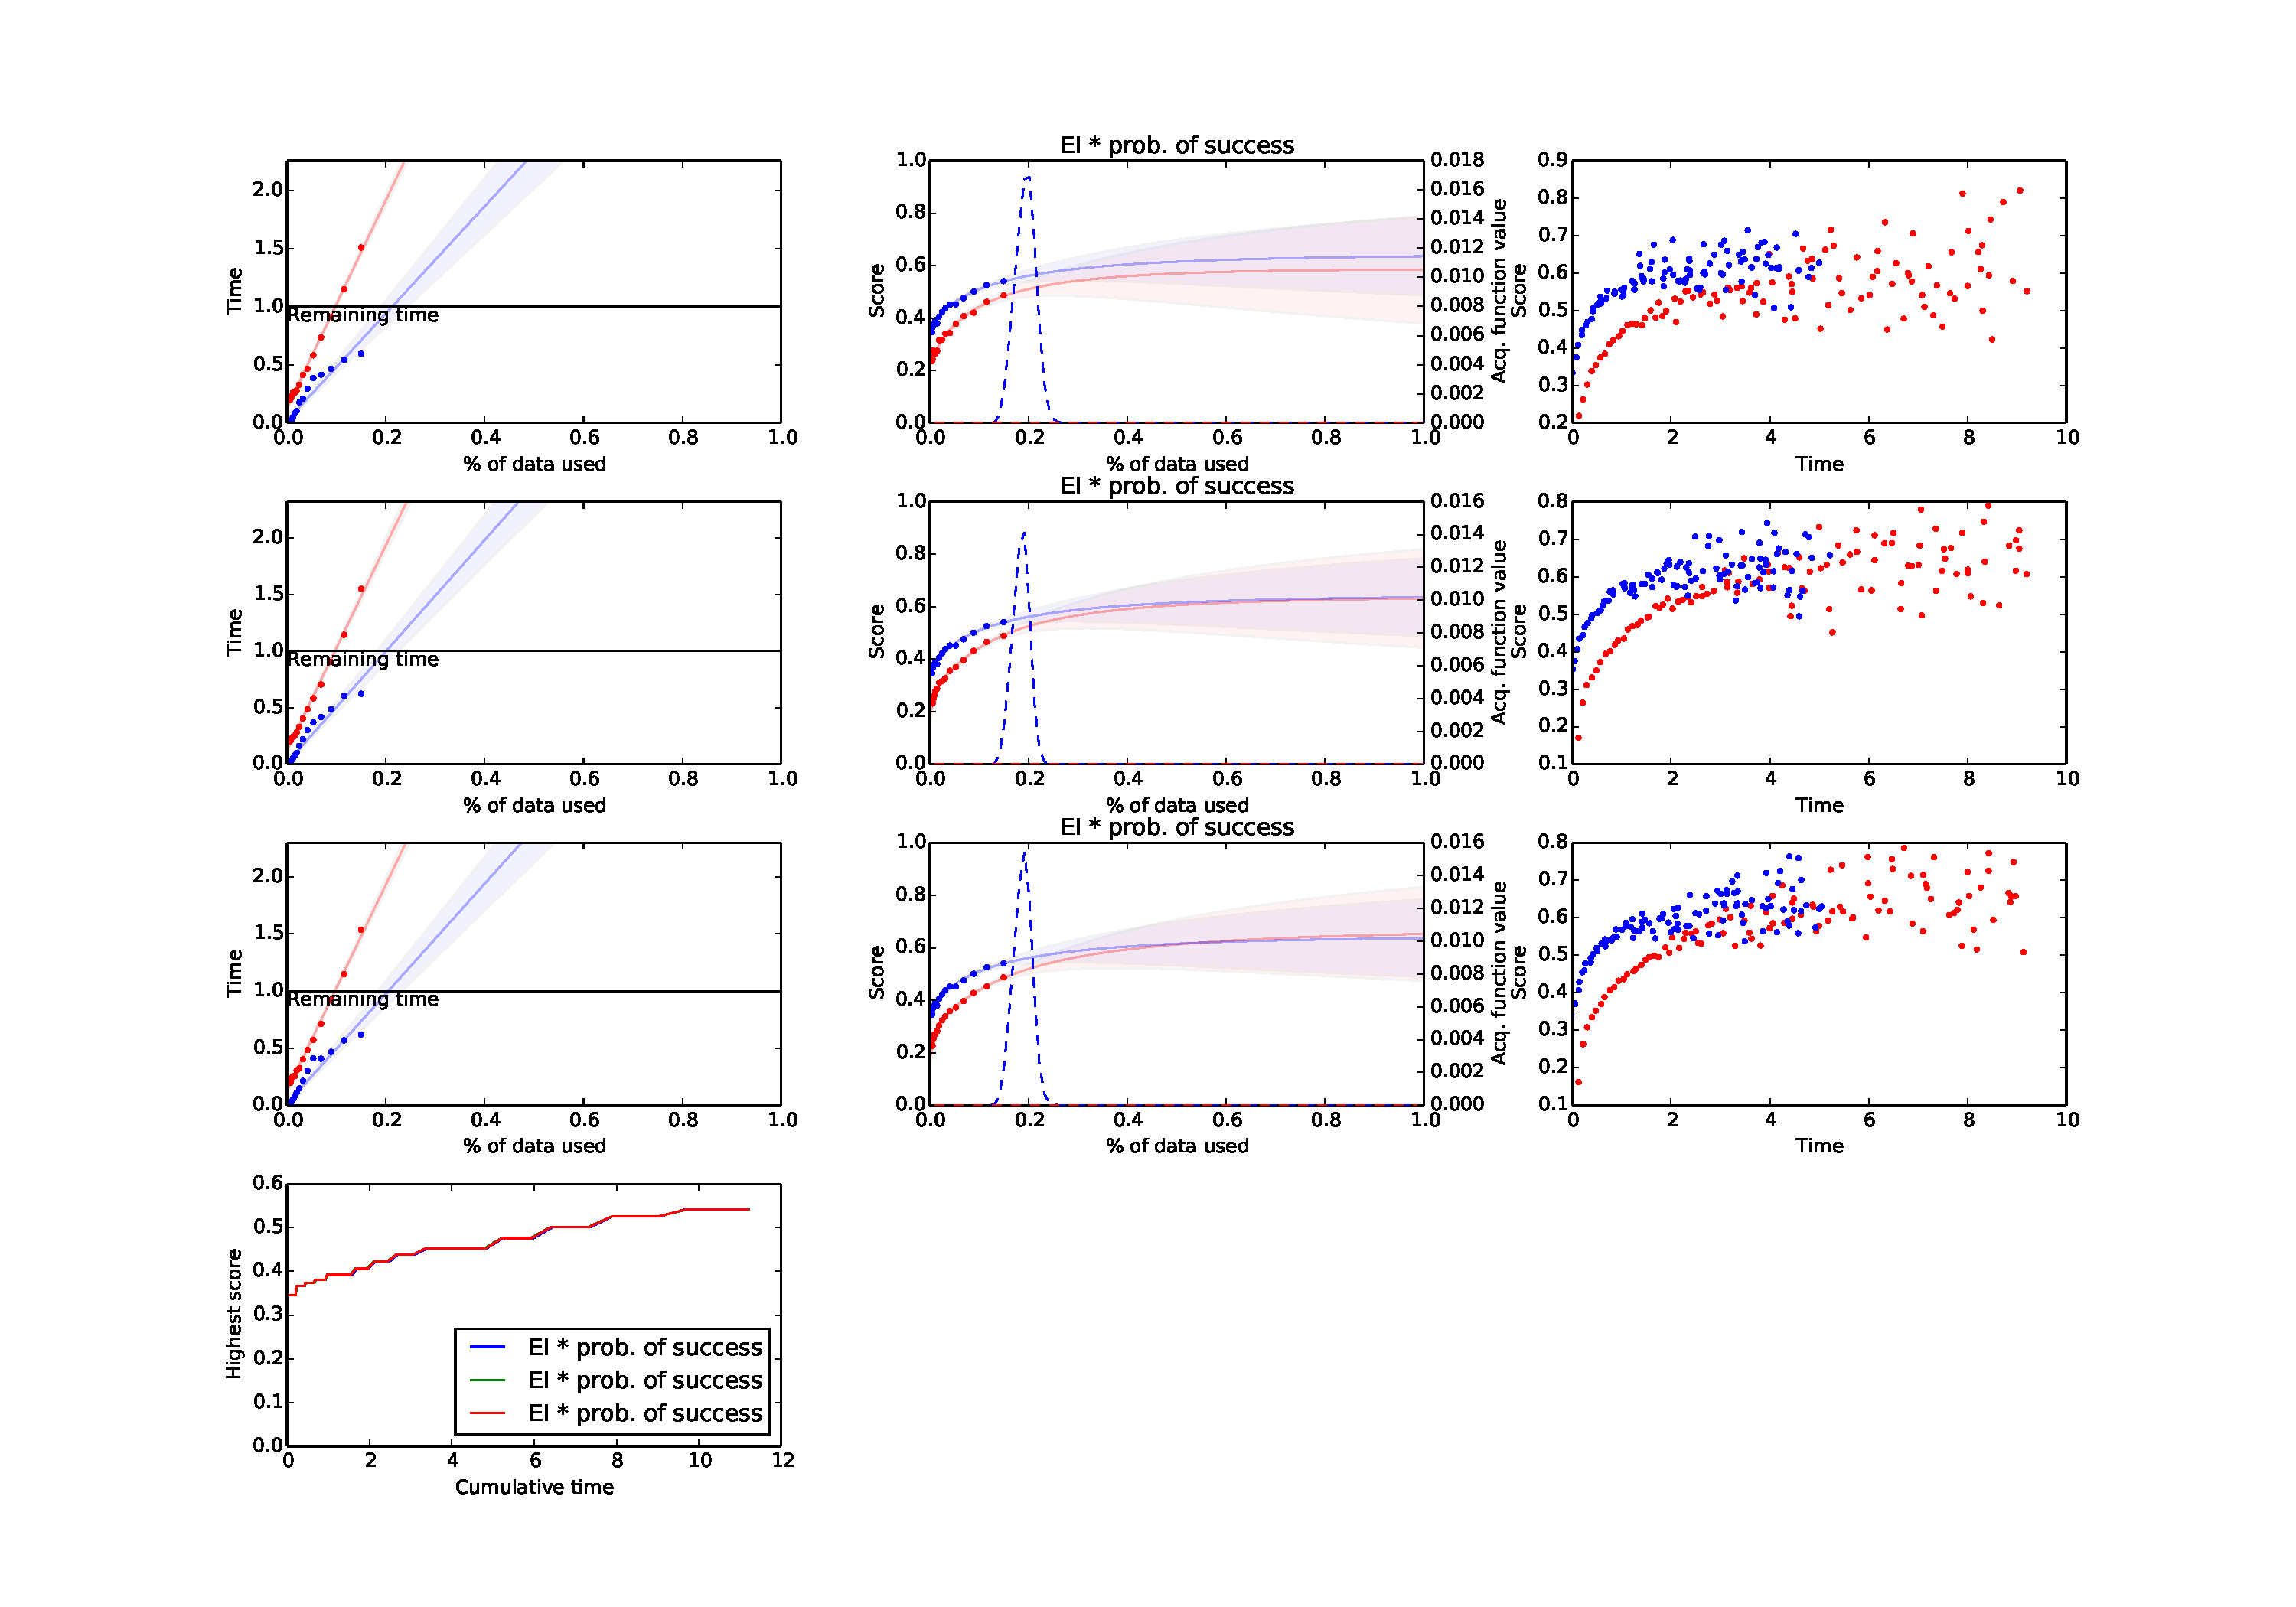
\includegraphics[trim=140 710 493 55,clip,width=\textwidth]{figures/ei_probofsuccess1.pdf}
  \caption{Expected improvement times probability of success after the burn in period with an initial time budget of one second}
  \label{sched:expimprpertime01}
\end{figure}

The acquisition function of the blue algorithm with its peak around 0.2 reflects that the fact that, although the running time of the blue algorithm grows slower, the time model predicts that evaluating the blue algorithm with 20\% of the data will take roughly one second. For values larger than that, the probability of success rapidly decreases.

\begin{figure}
\centering
  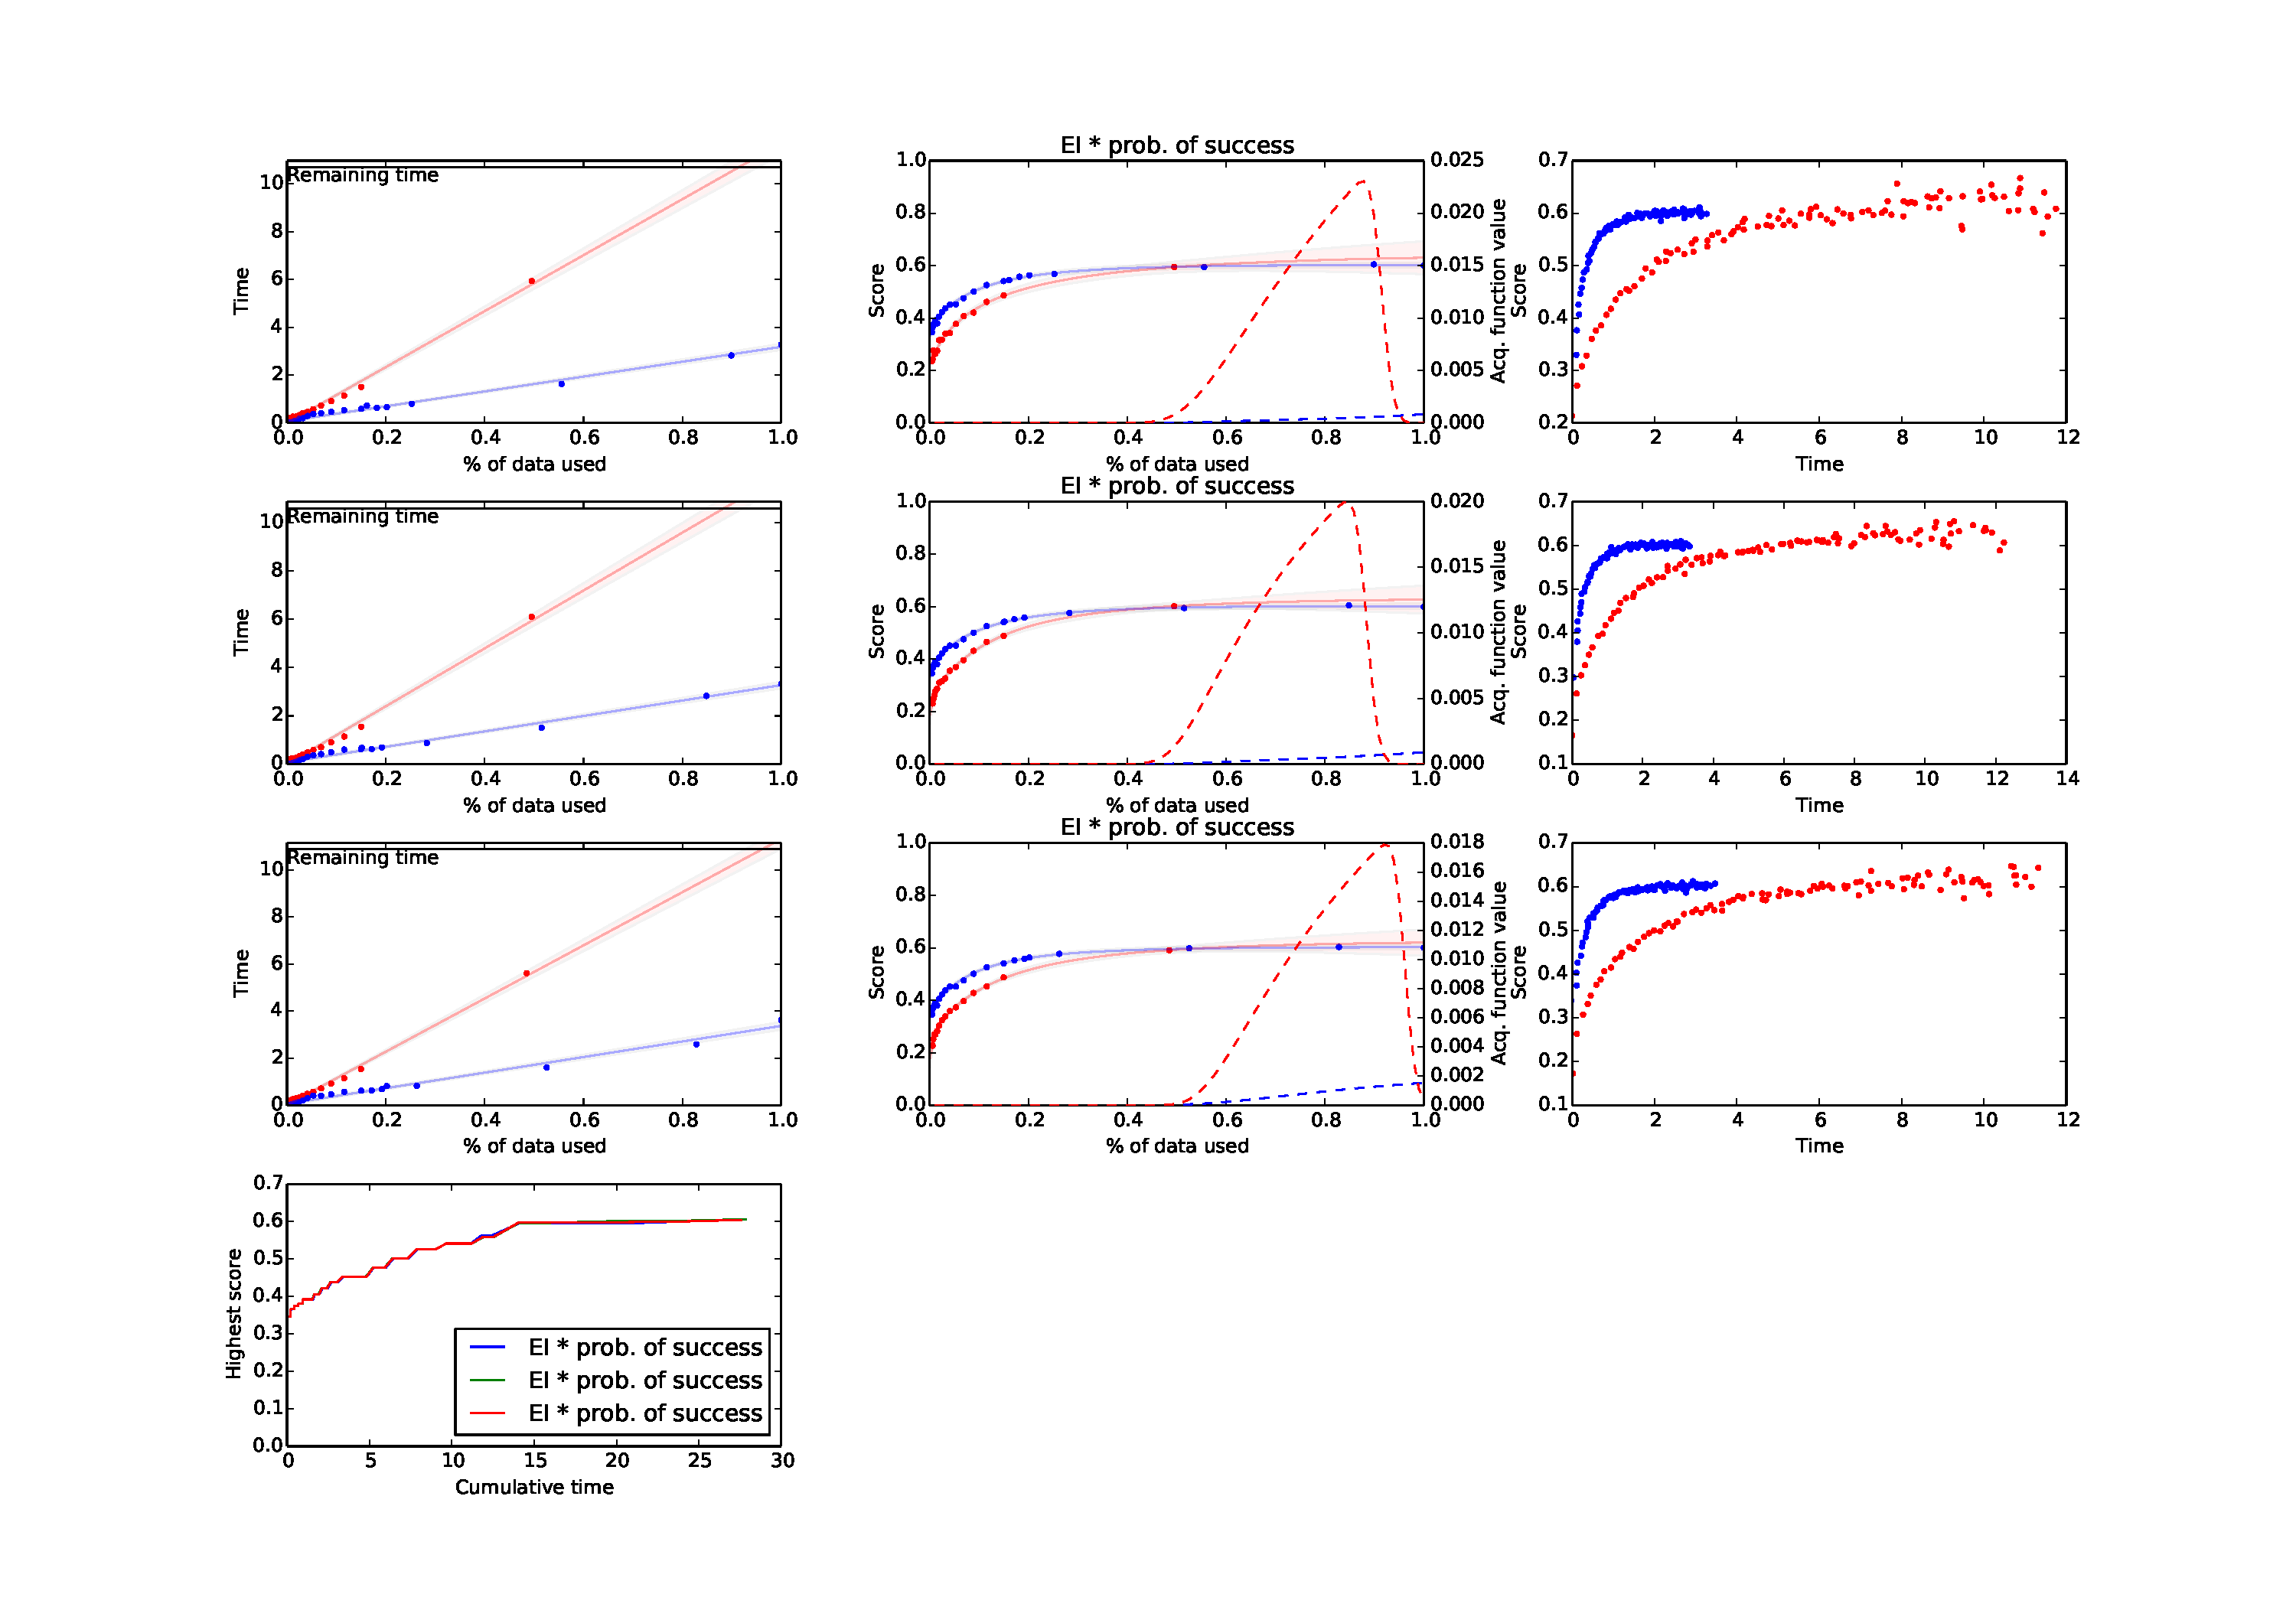
\includegraphics[trim=140 710 493 55,clip,width=\textwidth]{figures/ei_probofsuccess2.pdf}
  \caption{Expected improvement times probability of success}
  \label{sched:expimprpertime02}
\end{figure}

Figure \ref{sched:expimprpertime02} shows the \texttt{ExpectedImprovementTimesProbOfSuccessScheduler} at a later stage of execution. The blue algorithm has been evaluated at multiple points and the scheduler does not expect much improvement by evaluating it again at any point. The scheduler has about 12 seconds to spend on the red algorithm. The running time for this algorithm exceeds this limit for x values close to 1, which is reflected in the sharp drop off in the acquisition function on the right at around $0.9$.

\subsubsection{\texttt{MinimeseUncertaintyThenExploitScheduler}}
% TODO say what this scheduler is for (contract)

The \texttt{MinimeseUncertaintyThenExploitScheduler} is the most advanced scheduler implemented in this project. Although it fulfils a different purpose than the \texttt{ExpectedImprovementTimesProbOfSuccessScheduler} and can therefore not be compared to it directly, its behaviour is more complex and interesting. Recall that it functions in two stages, exploration and exploitation, that are each allocated a time budget.



% individual samples unimportant, only the overall variance

\begin{figure}
\centering
  \includegraphics[trim=140 710 493 55,clip,frame,width=\textwidth]{figures/exp_then_exp1.pdf}
  \caption{@@}
  \label{sched:eexp_then_exp1}
\end{figure}

\begin{figure}
\centering
  \includegraphics[trim=140 710 493 55,clip,width=\textwidth]{figures/exp_then_exp2.pdf}
  \caption{@@}
  \label{sched:exp_then_exp2}
\end{figure}

\begin{figure}
\centering
  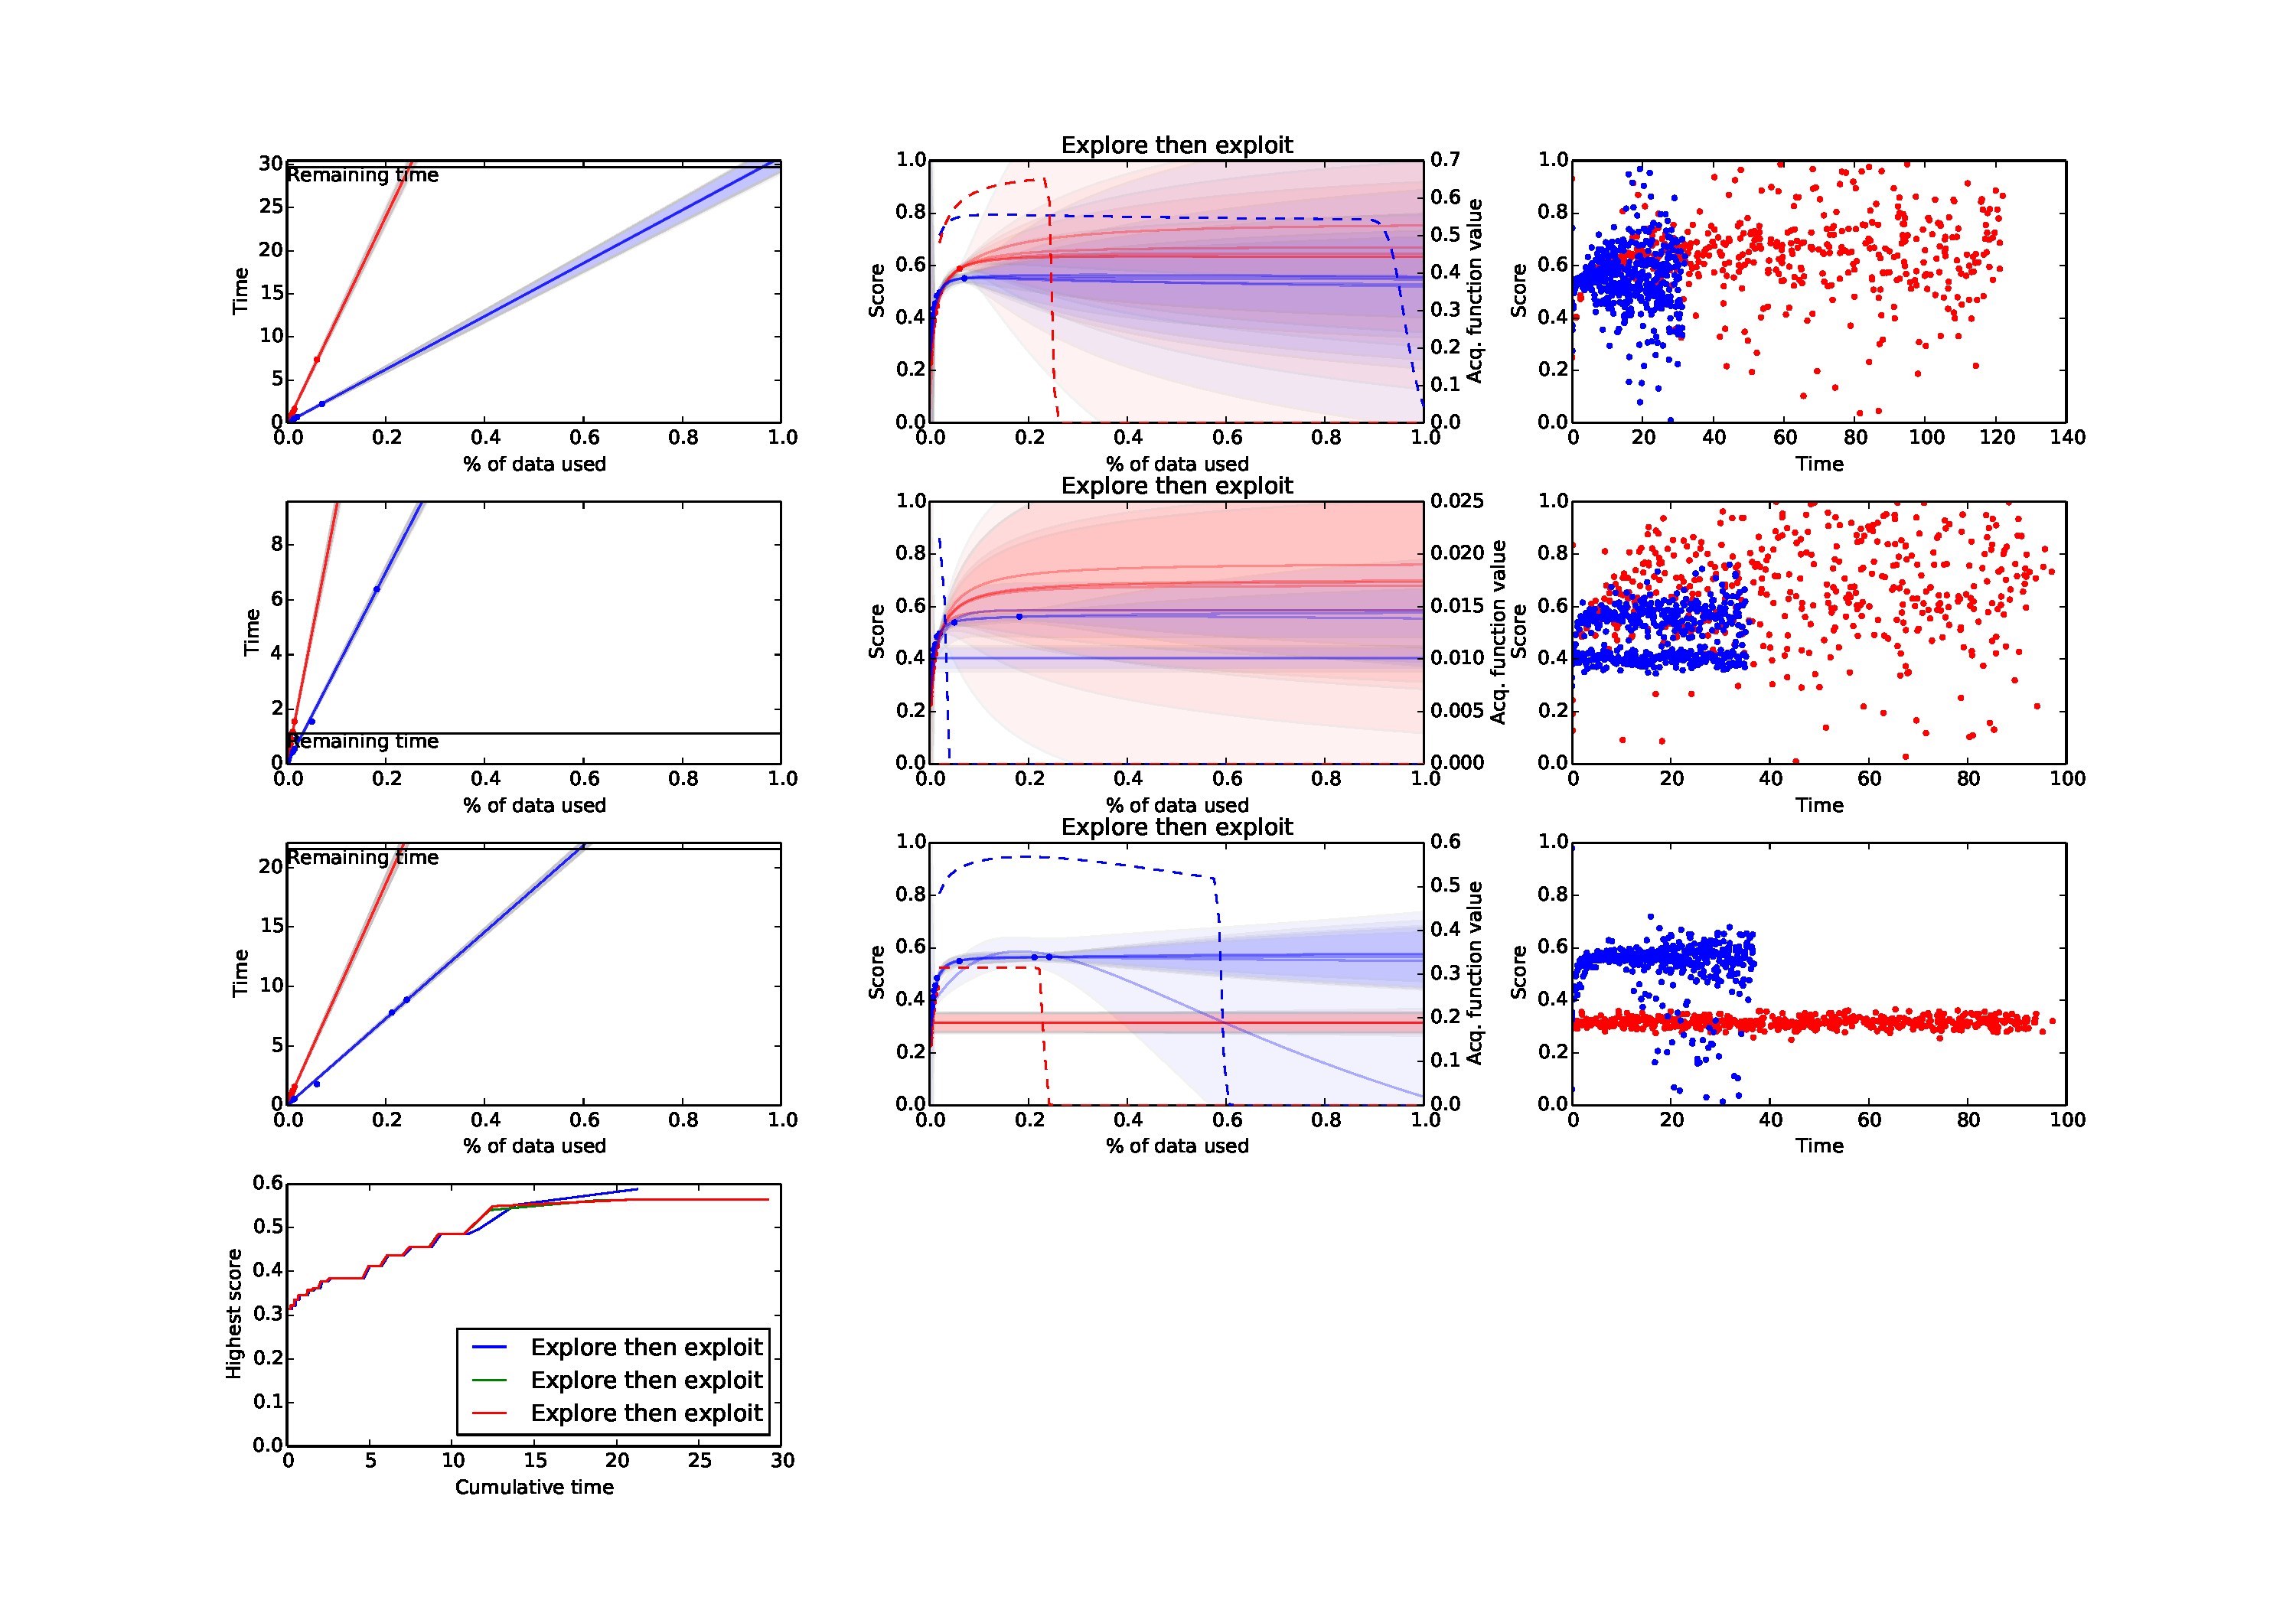
\includegraphics[trim=140 710 493 55,clip,width=\textwidth]{figures/exp_then_exp3.pdf}
  \caption{@@}
  \label{sched:exp_then_exp3}
\end{figure}



\subsection{Scheduler comparison}
In this section we will compare
% TOOD IMPLEMENT EI/time scheduler that gets fixed block of time

% TODO MAYBE write this
%\section{Limitations}


\section{Challenges}
One challenge we faced during the course of this problem which kept creating new problems resulted from our choice to implement our program in more than one programming languages. Python's \texttt{subprocess} library, which we used to call Matlab as described in section @@@, is far from intuitive and often caused zombie children of our main program to accumulate. 

Matlab, on the other side of our interoperability structure, is clearly not very well suited for reading and writing JSON data. Currently, we have to append an empty cell \texttt{\{\}} to a Matlab array that contains only one element when exporting it to prevent it from being exported as an individual object. This is an unsatisfying workaround to which the only true solution is to rewrite the Matlab code in Python.

Implementing the gradients of the hyperparameters to our kernel proved to be challenging. Even though we are not currently using them, we originally assumed we would use GPML's optimisation function which relies on gradient information. The difficulty of implementing them was compounded by the facts that kernels receive parameters in log space and that we reparameterised our kernel which made the derivative terms more complex.

To test our gradient implementation and ensure its correctness, we used a script provided by the creators of GPML that checks kernel gradients\footnote{This script can be downloaded at http://learning.eng.cam.ac.uk/carl/code/minimize/checkgrad.m}. % TODO maybe stress that they are correct

% TODO MAYBE move this somewhere else (data collection?)
% TODO ADD finish this
Another challenge we encountered during data collection for this project were unexplainable changepoints in the linear growth of running time. Figures \ref{time_dropoff1}, \ref{time_dropoff2} and \ref{time_dropoff3} show examples of this effect. Usually

This problem was very hard to investigate. We strongly suspect it to be explained by the particularities of the scikit-learn implementations and our computer specifications. It  disappeared when executing the same algorithm/parameter combinations on the EC2 instance and even on our local computer, small changes in hyperparameters often caused the problem to appear or disappear. Possible explanations would be an implementation that changes from one routine to another once some kind of threshold is reached or caching-related effects.

As this problem occurred rarely and did not have a noticeable impact on the performance of our system, we did not investigate it further.

% TODO mention sample sizes in all relevant places

\begin{figure}
\centering
% TODO FIGURE trim this to only show fixed sequence scheduler
  \includegraphics[trim=0 0 0 0,clip,width=\textwidth]{figures/time_dropoff1.pdf}
  \caption{@@@}
  \label{time_dropoff1}
\end{figure}
\begin{figure}
\centering
% TODO FIGURE trim this to only show fixed sequence scheduler
  \includegraphics[trim=0 0 0 0,clip,width=\textwidth]{figures/time_dropoff2.pdf}
  \caption{@@@}
  \label{time_dropoff2}
\end{figure}
\begin{figure}
\centering
% TODO FIGURE trim this to only show fixed sequence scheduler
  \includegraphics[trim=0 0 0 0,clip,width=\textwidth]{figures/time_dropoff3.pdf}
  \caption{@@@}
  \label{time_dropoff3}
\end{figure}



% TODO numerical accuracy for EI when sd is very small and peak is under lower bound, i.e. prob of impr is very small, get infs and nans
% TODO "hinge" on my computer


\chapter{Conclusion and future work} 
% TODO finish this chapter
\section{Conclusions}
In this project, we have succeeded in
\begin{itemize}
	\item creating a covariance function for Gaussian processes that model the exponential behaviour of learning algorithm accuracy as a function of appoximation parameters
	\item developing heuristics that make use of this kernel to create models under run time constraints
\end{itemize}


\section{Future work}
One straightforward way our system could be extended is by considering more algorithms beside logistic regression and random forest. Scikit-learn contains implementations of a great number of other machine learning algorithms that could be added to the current list of algorithms with little additional work. One challenge in this is to make the graphical output of the program stay readable while more models and lines are added.

Similarly, the program could be extended to consider additional hyperparameters besides the percentage of data. This would likely require entirely new ways of visualising the output as it is very difficult to plot functions that take more than one argument.

% TODO turn this into a paragraph
Greedy strategies such as those implemented as schedulers in this project are not optimal. This is 

% TODO additional appr params. the kernel is already implemented

% TODO Depending on the length of your work, and  how well you write, you may not need a summary here. You will generally want to draw some conclusions, and point to potential future work. 
% TODO transfer learning? to avoid burn in



\appendix
\singlespacing

% TODO ADD more references

\bibliographystyle{unsrt} 
\bibliography{references}


\end{document}
